\documentclass[12pt,a4paper]{article}
\usepackage[utf8]{inputenc}
\usepackage[T1]{fontenc}
\usepackage[english,bahasa]{babel}
\usepackage{amsmath}
\usepackage{amsfonts}
\usepackage{amssymb}
\usepackage{graphicx}
\usepackage{geometry}
\usepackage{setspace}
\usepackage{hyperref}
\usepackage{booktabs}
\usepackage{array}
\usepackage{xcolor}
\usepackage{enumitem}
\usepackage{titlesec}
\usepackage{fancyhdr}
\usepackage{lastpage}
\usepackage{titling}
\usepackage{float}
\usepackage{lmodern}
\usepackage{booktabs}
\usepackage{tabularx}
\usepackage{booktabs}
\usepackage{longtable}
\usepackage{array}
\usepackage{listings}
\usepackage{xcolor}
\usepackage{tcolorbox}
\usepackage{newunicodechar}
\tcbuselibrary{listings, breakable}

% Container ASCII setup
\newtcblisting{asciiBox}{
    listing only,
    listing options={
        basicstyle=\ttfamily\small,
        breaklines=true,
        columns=fullflexible,
        keepspaces=true
    },
    colback=white,
    colframe=black,
    arc=2pt,
    boxrule=0.4pt,
    breakable
}

% Container code setup
\definecolor{vscodeBackground}{HTML}{1E1E1E}
\definecolor{vscodeText}{HTML}{D4D4D4}
\definecolor{vscodeKeyword}{HTML}{569CD6}
\definecolor{vscodeString}{HTML}{CE9178}
\definecolor{vscodeComment}{HTML}{6A9955}
\definecolor{vscodeNumber}{HTML}{B5CEA8}

\lstdefinestyle{vscode}{
  backgroundcolor=\color{vscodeBackground},
  basicstyle=\ttfamily\footnotesize\color{vscodeText},
  keywordstyle=\color{vscodeKeyword},
  stringstyle=\color{vscodeString},
  commentstyle=\color{vscodeComment}\itshape,
  numberstyle=\tiny\color{gray},
  numbers=left,
  numbersep=8pt,
  frame=single,
  rulecolor=\color{gray!70},
  showstringspaces=false,
  breaklines=true,
  tabsize=2,
  captionpos=b,
}

% Set margin dan spacing
\geometry{a4paper, top=2.5cm, bottom=2.5cm, left=2.5cm, right=2.5cm}
\setstretch{1.0}

% Hyperlink setup
\hypersetup{
    colorlinks=true,
    linkcolor=black,
    filecolor=magenta,      
    urlcolor=cyan,
    citecolor=blue
}

% Format section
\titleformat{\section}{\normalfont\Large\bfseries}{\thesection}{1em}{}
\titleformat{\subsection}{\normalfont\large\bfseries}{\thesubsection}{1em}{}
\titleformat{\subsubsection}{\normalfont\normalsize\bfseries}{\thesubsubsection}{1em}{}

% Header and footer
\pagestyle{fancy}
\fancyhf{}
\fancyhead[L]{
    \raisebox{-0.35cm}{
        
\includegraphics[height=1.2cm]{img/itb.png}\hspace{0.3cm}
        
\includegraphics[height=1.2cm]{img/stei-itb.jpg}\hspace{0.3cm}
        
\includegraphics[height=1.2cm]{img/lab-irk.jpg}
    }
}
\fancyhead[R]{
    \parbox{8cm}{
        \raggedleft
        \footnotesize \textbf{IF2123 Aljabar Linier dan Geometri}\\
        \footnotesize Laporan Tugas Besar 2\\
        \footnotesize \emph{Semester I 2025/2026}
    }
}
\fancyfoot[R]{Halaman \thepage\ dari \pageref{LastPage}}

\renewcommand{\headrulewidth}{0.2pt}
\renewcommand{\footrulewidth}{0.2pt}

\setlength{\headheight}{1.5cm}
\setlength{\headsep}{0.8cm}

\fancypagestyle{plain}{
    \fancyhf{}
    \fancyfoot[C]{\footnotesize Halaman \thepage\ dari \pageref{LastPage}}
    \renewcommand{\headrulewidth}{0pt}
    \renewcommand{\footrulewidth}{0.4pt}
}

\geometry{a4paper, top=3.5cm, bottom=2.5cm, left=2.5cm, right=2.5cm, headheight=1.5cm, headsep=0.8cm}

\begin{document}

% Cover 
\begin{titlepage}
    \pagestyle{empty}
    \centering

    {\Large \textbf{ Laporan Tugas Besar 2}}
    \vspace{0.70em}
    
    \setstretch{1.0}
    {\large \textsc{ IF2123 Aljabar Linear dan Geometri}}
    \vspace{0.25em}
    
    {\textsc{Sistem Persamaan Linier, Determinan, dan Penerapannya}}
    \vspace{0.25em}
    
    {\small \textsc{Semester I Tahun 2025/2026}}
    \vspace{1.5cm}
    
    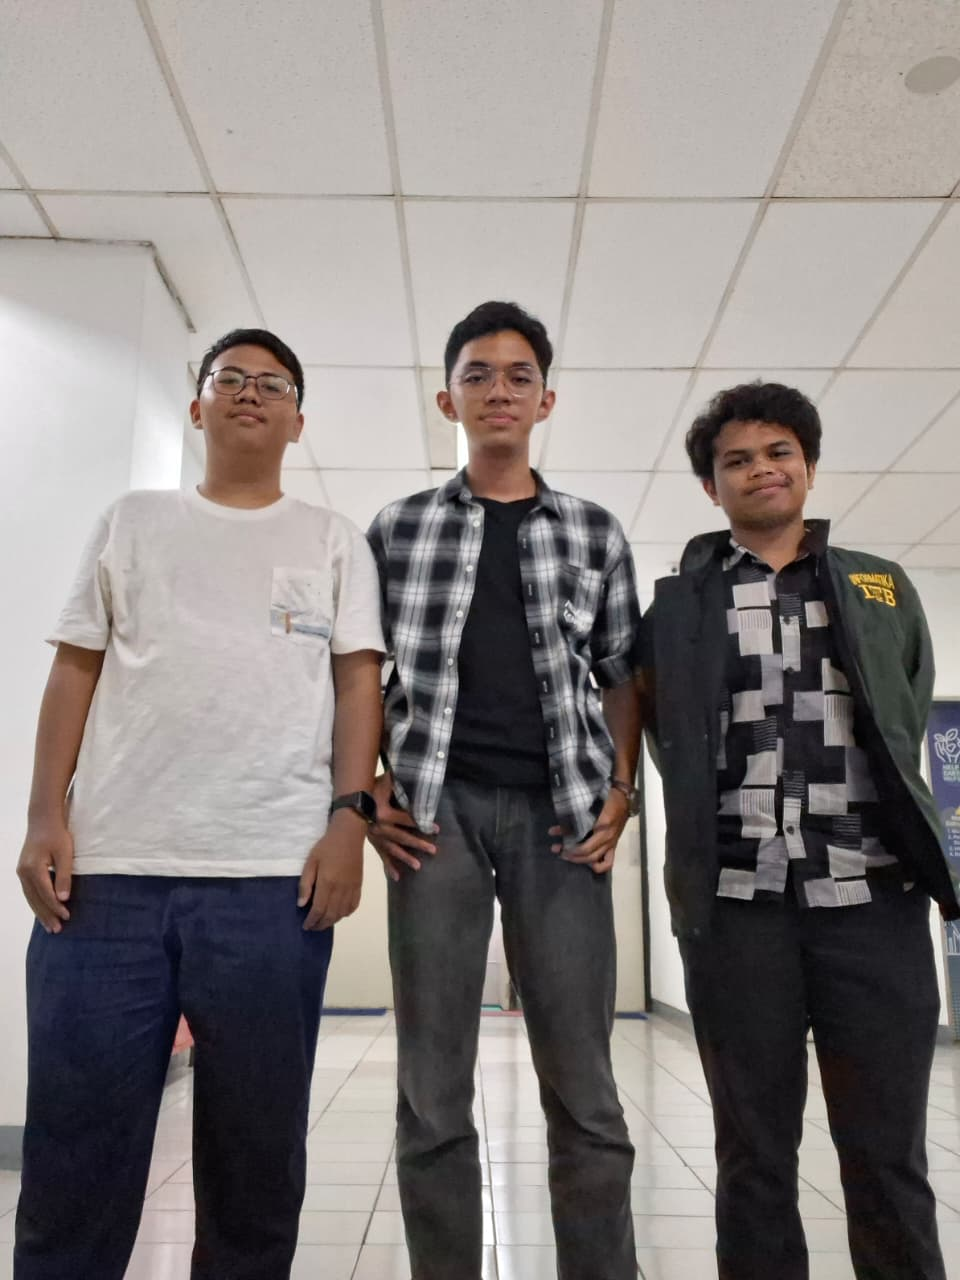
\includegraphics[width=0.5\textwidth]{img/foto_kelompok.jpg}\\
    \vspace{1cm}
    
    \begin{spacing}{1.0}
    {\large {\textsc{E-Tanol}}}
    \vspace{0.5cm}
    
    {\textsc{Anggota:}}
    \vspace{0.3cm}
    
    \begin{tabular}{c}
        An-Dafa Anza Avansyah (13524038) \\
        Muhammad Haris Putra Sulastianto (13524053) \\
        Fazri Arrashyi Putra (13524127) \\
    \end{tabular}
    \vspace{1.5cm}
    \end{spacing}
    
    { \textsc {Laboratorium Ilmu dan Rekayasa Komputasi}}
    \vspace{0.25em}
    
    {\textsc {Program Studi Teknik Informatika}}
    \vspace{0.25em}
    
    {\textsc {Sekolah Teknik Elektro dan Informatika}}
    \vspace{0.25em}
    
    {\textsc {Institut Teknologi Bandung}}
    \vspace{0.25em}
    
    {\textsc{ \today}}
\end{titlepage}

% Reset spacing untuk konten
\setstretch{1.0}

% Daftar Isi
\addtocontents{toc}{\protect\setcounter{tocdepth}{3}}
\tableofcontents
\newpage

% Daftar Gambar
\listoffigures
\newpage

% Daftar Tabel
\listoftables
\newpage

% Daftar Listing
% \lstlistoflistings
% \newpage

% Header bab selanjutnya
\pagestyle{fancy}

% BAB 1 PENDAHULUAN
\section{Pendahuluan}

\subsection{Kisah}
\small
Di Desa Konohagakure, hiduplah dua orang mahasiswa Teknik Informatika bernama Ayu dan Asep
Kasep. Akhir-akhir ini, Ayu merasa kewalahan memahami materi dekomposisi matriks yang diajarkan
dalam mata kuliah IF2123 Aljabar Linier dan Geometri karena ketimbang memperhatikan penjelasan
dosen di depan, ia malah asyik doomscrolling di media sosial. Supaya bisa bertanggung jawab kepada
kedua orang tuanya yang telah membiayai kuliahnya, Ayu pun bertekad untuk memperbaiki situasi
dengan belajar ke perpustakaan. Sesampainya di sana, ia takjub akan banyaknya koleksi buku yang
tersedia. Sejak saat itu, Ayu pun gemar mengunjungi perpustakaan untuk mengeksplorasi berbagai
macam buku yang menarik minatnya.

Di sisi lain, Asep adalah seorang mahasiswa yang bekerja paruh waktu sebagai pustakawan di perpustakaan
kampus. Sejak Ayu mulai rajin berkunjung ke perpustakaan, Asep sering membantunya mencari
buku-buku yang diinginkannya. Awalnya, Ayu mengira Asep adalah seorang performative male yang
hanya ingin pamer di hadapannya. Apalagi, Asep sering sekali minum matcha. Namun, seiring berjalannya
waktu, Ayu menyadari bahwa Asep adalah sosok yang cerdas dan tulus dalam membantu sesama. Asep juga sadar bahwa Ayu adalah pribadi yang tekun dan pantang menyerah. Akhirnya, mereka pun
jatuh cinta.

\begin{figure}[H]
    \centering
    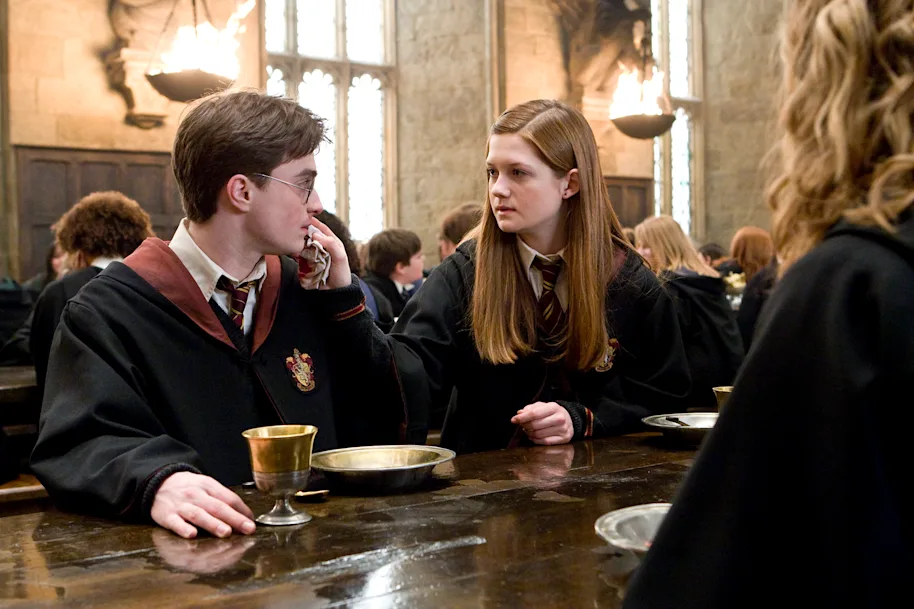
\includegraphics[width=0.75\textwidth]{img/Asep-Ayu.jpg}
    \caption{Anggaplah ini Ayu dan Asep.}
    \label{fig:asep-ayu}
\end{figure}

Asep menyadari bahwa Ayu sering kali kesulitan menemukan buku yang diinginkannya atau melan-
jutkan bacaan dari buku yang pernah dipinjamnya sebelumnya. Hal ini dikarenakan sistem pencarian buku di perpustakaan yang masih konvensional dan kurang efisien. Melihat hal tersebut, Asep terinspirasi untuk mengembangkan sebuah sistem temu balik informasi berbasis singular value decomposition (SVD) dan vektor eigen yang dapat membantu Ayu dan pengunjung perpustakaan lainnya dalam menemukan buku dengan lebih mudah dan cepat. 

Untuk membuktikan bahwa mahasiswa Teknik Informatika memanglah solid, mari kita bantu Asep dalam merancang dan mengimplementasikan sistem temu balik informasi tersebut dengan memanfaatkan konsep-konsep aljabar linier yang telah kita pelajari di mata kuliah IF2123 Aljabar Linier dan Geometri.

\subsection{Tujuan}
Pada Tugas Besar 2 ini, kita akan mengembangkan sebuah aplikasi web untuk sistem perpustakaan digital. Anda akan diberikan sebuah dataset berisi koleksi buku dengan rincian judul, konten (berupa file txt), dan sampul (berupa file jpg). Aplikasi ini harus mampu menampilkan daftar buku dalam dataset dengan 
\href{https://developer.mozilla.org/en-US/docs/Web/CSS/How_to/Layout_cookbook/Pagination}{paginasi}, menampilkan konten buku untuk dibaca, melakukan pencarian buku berdasarkan input sampul gambar dari penggunaan atau kata kunci teks dari pengguna, serta memberikan rekomendasi buku yang relevan berdasarkan buku yang sedang dibaca.

% BAB 2 DASAR TEORI
\newpage
\section{Dasar Teori}

\subsection{\textit{Eigen Value} dan \textit{Eigen Vector}}
\subsubsection{Teori Singkat}

Dalam materi aljabar linier \cite{algeo2025}, jika $A$ adalah sebuah matriks persegi berukuran $n \times n$, maka sebuah vektor tak-nol $x$ di $R^n$ disebut sebagai vektor eigen dari $A$ jika perkalian $A$ dengan $x$ menghasilkan vektor yang merupakan kelipatan skalar dari $x$ itu sendiri.\\

\noindent Hubungan ini dituliskan dalam persamaan fundamental:
$$Ax = \lambda x$$

\noindent Dimana:
\begin{itemize}[label=\textbullet]
    \item $x$ adalah vektor eigen (tidak boleh nol).
    \item $\lambda$ (lambda) adalah skalar yang disebut nilai eigen dari $A$.
\end{itemize}

Kata "eigen" sendiri berasal dari Bahasa Jerman yang berarti "asli" atau "karakteristik", sehingga nilai eigen sering juga disebut sebagai nilai karakteristik dari sebuah matriks

\subsubsection{Makna Geometris}

Secara geometris, perkalian matriks $A$ dengan vektor biasa umumnya akan mengubah arah dan panjang vektor tersebut (rotasi dan skala). Namun, untuk vektor eigen, perkalian dengan matriks $A$ tidak mengubah arah garis vektor tersebut, melainkan hanya mengubah panjangnya (skala).

\begin{figure}[H]
    \centering
    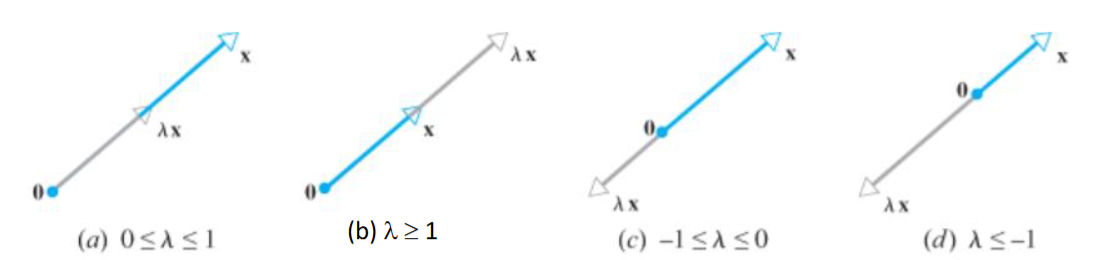
\includegraphics[width=1\linewidth]{img/vector-lambda.png}
    \caption{Vektor $x$ menyusut atau memanjang dengan faktor $\lambda$}
    \label{fig:vector-with-lambda-factor}
\end{figure}

\begin{itemize}[label=\textbullet]
    \item Operasi $Ax = \lambda x$ menyebabkan vektor $x$ memanjang atau menyusut dengan faktor skala $\lambda$.
    \item Jika $\lambda > 0$, vektor hasil memiliki arah yang sama dengan $x$.
    \item Jika $\lambda < 0$, vektor hasil memiliki arah yang berkebalikan dengan $x$.
    \item Jika $\lambda = 1$, vektor tidak berubah panjang maupun arah.
\end{itemize}

\subsubsection{Metode Komputasi Numerik: Power Iteration \& Deflation}

Dalam teori dasar aljabar linier, nilai eigen biasanya dicari menggunakan persamaan karakteristik $\det(\lambda I - A) = 0$. Namun, metode ini memiliki kompleksitas komputasi yang sangat tinggi ($O(n^3)$ atau lebih) dan tidak efisien untuk matriks berukuran besar seperti data citra atau teks yang memiliki ribuan dimensi.Oleh karena itu, dalam implementasi tugas besar ini, digunakan pendekatan numerik iteratif yang lebih efisien:\\

\begin{enumerate}
    \item Power Iteration (Metode Pangkat) {
    \newline Power Iteration adalah algoritma iteratif untuk menemukan nilai eigen mutlak terbesar ($\lambda_{max}$) dan vektor eigen yang bersesuaian dari sebuah matriks. Metode ini bekerja dengan prinsip bahwa jika sebuah vektor acak dikalikan berulang kali dengan matriks $A$, vektor tersebut akan perlahan berkonvergensi ke arah vektor eigen dominan.Algoritma Power Iteration yang diimplementasikan adalah sebagai berikut:
    \begin{enumerate}
        \item Inisialisasi vektor acak $b_0$ dengan norma 1
        \item Lakukan iterasi untuk $k = 1, 2, \dots$: {
            Hitung vektor baru: $\tilde{b}_{k+1} = A b_k$. Normalisasi vektor: $b_{k+1} = \frac{\tilde{b}_{k+1}}{||\tilde{b}_{k+1}||}$
        }
        \item Nilai eigen $\lambda$ didekati menggunakan Rayleigh Quotient:$$\lambda = \frac{b_k^T A b_k}{b_k^T b_k}$$ 
    \end{enumerate}
    }

    \item Hotelling's Deflation (Metode Deflasi) {\newline Power Iteration hanya dapat menemukan satu nilai eigen terbesar. Untuk menemukan nilai eigen kedua, ketiga, dan seterusnya (sebanyak $k$ komponen utama), digunakan teknik Deflasi.Setelah pasangan nilai eigen ($\lambda_1$) dan vektor eigen ($v_1$) ditemukan, kontribusi mereka "dihilangkan" dari matriks asal $A$ agar iterasi berikutnya dapat menemukan nilai eigen terbesar berikutnya. Rumus deflasi yang digunakan adalah:$$A_{baru} = A - \lambda_1 v_1 v_1^T$$ Proses Power Iteration kemudian diulang pada matriks $A_{baru}$ ini.
    }
\end{enumerate}

\subsection{\textit{Singular Value Decomposition }(SVD)}
\subsubsection{Teori Singkat}
Singular Value Decomposition (SVD) adalah metode untuk memfaktorkan sembarang matriks (baik persegi maupun non-persegi berukuran $m \times n$).\\

\noindent Rumus dekomposisi SVD adalah:
$$A = U \Sigma V^T$$
Dimana komponen-komponennya adalah:
\begin{itemize}
    \item $A$: Matriks asal ($m \times n$).
    \item $U$: Matriks ortogonal ($m \times m$). Kolom-kolomnya disebut vektor singular kiri.
    \item $\Sigma$ (Sigma): Matriks diagonal ($m \times n$) yang berisi nilai-nilai singular ($\sigma$). Nilai ini selalu positif dan diurutkan dari besar ke kecil.
    \item $V^T$: Transpose dari matriks ortogonal $V$ ($n \times n$). Kolom-kolom $V$ disebut vektor singular kanan.
\end{itemize}

\subsubsection{Cara Menghitung SVD}
Ada dua cara umum untuk menghitung komponen SVD yang dijelaskan dalam materi aljabar linier dan geometri\cite{algeo2025}.\\

\noindent \textbf{Langkah Utama}
\begin{enumerate}
    \item Cari $V$ (Vektor Singular Kanan):
    \begin{itemize}
        \item Hitung matriks $A^T A$.
        \item Cari nilai eigen ($\lambda$) dan vektor eigen dari $A^T A$.
        \item Normalisasi vektor eigen tersebut menjadi panjang satuan (dibagi panjangnya). Vektor-vektor ini membentuk matriks $V$.
    \end{itemize}
    \item Cari $\Sigma$ (Nilai Singular):
    \begin{itemize}
        \item Nilai singular ($\sigma$) adalah akar kuadrat dari nilai eigen $A^T A$ ($\sigma_i = \sqrt{\lambda_i}$).
        \item Susun $\sigma$ pada diagonal utama matriks $\Sigma$ dari terbesar ke terkecil.
    \end{itemize}
    \item Cari $U$ (Vektor Singular Kiri):
    \begin{itemize}
        \item Gunakan rumus hubungan: $u_i = \frac{1}{\sigma_i} A v_i$.
        \item Jika jumlah vektor $u$ belum memenuhi ukuran matriks $U$ (karena $m > n$), lakukan perluasan basis ortonormal (Gram-Schmidt) untuk melengkapinya.
    \end{itemize}
\end{enumerate}

\noindent \textbf{Langkah Alternatif}
\begin{itemize}
    \item Cari $U$ dengan menghitung vektor eigen dari $A A^T$.
    \item Cari $V$ dengan menghitung vektor eigen dari $A^T A$.
\end{itemize}

\subsubsection{SVD Tereduksi (\textit{Reduced} SVD)}
Seringkali matriks $\Sigma$ memiliki banyak angka nol (terutama jika $m \neq n$). Kita bisa "membuang" baris atau kolom nol tersebut untuk menghemat tempat.
Bentuk ini disebut SVD Tereduksi:
$$A = U_1 \Sigma_1 V_1^T$$
Dimana ukurannya lebih kecil (\textit{compact}) namun tetap menghasilkan matriks $A$ yang sama persis.

\subsubsection{Aplikasi SVD}
Salah satu aplikasi utama SVD yang disebutkan dalam materi adalah Pemampatan Citra (\textit{Image Compression}).
\begin{itemize}
    \item Prinsipnya: Citra digital adalah matriks.
    \item Dengan SVD, kita bisa mengambil hanya beberapa nilai singular terbesar ($k$ teratas) dan membuang sisanya yang kecil (dianggap noise atau kurang penting).
    \item Hasilnya adalah citra yang ukurannya jauh lebih kecil (dikompresi) namun secara visual masih mirip dengan aslinya.
\end{itemize}

\subsection{Principal Component Analysis (PCA)}
\textit{Principal Component Analysis} (PCA) adalah teknik reduksi dimensi statistik yang digunakan untuk menyederhanakan kompleksitas data berdimensi tinggi dengan tetap mempertahankan tren dan pola informasi yang paling penting.

\subsubsection{Prinsip Dasar: Variansi sebagai Informasi}
Inti dari PCA adalah konsep variansi (penyebaran data). Dalam pengolahan citra, variansi yang tinggi antar piksel diasumsikan mengandung informasi struktur yang penting (seperti bentuk wajah atau garis tepi objek), sedangkan variansi rendah dianggap sebagai \textit{noise} atau latar belakang yang seragam.

PCA bekerja dengan melakukan transformasi linear untuk memproyeksikan data asli ke dalam sistem koordinat baru. Sumbu-sumbu baru ini disebut \textit{Principal Components} (PC) atau Komponen Utama, yang memiliki sifat:

\begin{enumerate}
    \item PC Pertama: Mengarah pada variansi data terbesar.
    \item PC Kedua: Tegak lurus (ortogonal) terhadap PC pertama dan menangkap variansi terbesar kedua, dan seterusnya.
\end{enumerate}

\subsubsection{Hubungan dengan SVD dan Eigenface}
Dalam implementasi sistem ini, PCA tidak selalu dihitung melalui dekomposisi matriks kovarian secara eksplisit (karena komputasi yang berat), melainkan sering kali dihitung menggunakan SVD.

Jika matriks data citra $\mathbf{X}$ telah dipusatkan (\textit{mean-centered}), maka vektor singular kiri ($\mathbf{U}$) dari hasil SVD matriks $\mathbf{X}$ adalah vektor-vektor komponen utama (\textit{Principal Components}) itu sendiri. Dalam konteks pengenalan wajah, vektor-vektor ini disebut \textit{Eigenfaces}.

$$\mathbf{X} = \mathbf{U} \mathbf{\Sigma} \mathbf{V}^T$$

Di mana kolom-kolom $\mathbf{U}$ adalah "wajah dasar" yang merepresentasikan fitur visual utama dari seluruh \textit{dataset}.

\subsection{Latent Semantic Analysis (LSA)}
\textit{Latent Semantic Analysis} (LSA), atau sering juga disebut \textit{Latent Semantic Indexing} (LSI), adalah teknik dalam Pemrosesan Bahasa Alami (\textit{Natural Language Processing}) untuk menganalisis hubungan antara sekumpulan dokumen dan istilah-istilah (kata) yang terkandung di dalamnya.

\subsubsection{Konsep Semantik Laten}
Masalah utama dalam pencarian teks sederhana (\textit{keyword matching}) adalah:
\begin{enumerate}
    \item Sinonim: Dua kata berbeda bisa memiliki makna sama (contoh: "mobil" dan "kendaraan").
    \item Polisemi: Satu kata bisa memiliki banyak makna tergantung konteks.
\end{enumerate}
LSA mengatasi ini dengan tidak mencocokkan kata secara mentah, melainkan memetakan kata dan dokumen ke dalam "ruang konsep laten" (\textit{latent semantic space}). Dokumen yang membahas topik serupa akan berdekatan dalam ruang ini meskipun tidak menggunakan kata-kata yang persis sama.

\subsubsection{Representasi Matematis}
LSA dimulai dengan membangun \textit{Term-Document Matrix} ($\mathbf{A}$), di mana baris merepresentasikan kata (\textit{terms}) dan kolom merepresentasikan dokumen. Nilai sel $A_{ij}$ biasanya diisi dengan bobot frekuensi kata (seperti TF-IDF).

LSA kemudian menerapkan SVD Tereduksi (\textit{Truncated SVD}) pada matriks $\mathbf{A}$:

$$\mathbf{A}_k = \mathbf{U}_k \mathbf{\Sigma}_k \mathbf{V}_k^T$$

\begin{itemize}
    \item $\mathbf{U}_k$ (Term Space): Merepresentasikan hubungan antara kata dengan topik laten.
    \item $\mathbf{V}_k^T$ (Document Space): Merepresentasikan hubungan antara dokumen dengan topik laten.
    \item $\mathbf{\Sigma}_k$: Menunjukkan kekuatan atau signifikansi dari setiap topik laten tersebut.
\end{itemize}

Dengan mengambil hanya $k$ nilai singular terbesar (\textit{aproksimasi low-rank}), LSA menghilangkan "gangguan" (\textit{noise}) dari variasi penggunaan kata yang tidak penting, sehingga mampu menangkap esensi semantik dari dokumen tersebut.

\subsection{Jawaban Pertanyaan Asisten}
\subsubsection{Mengapa SVD lebih cocok dibandingkan Eigendecomposition?}
Dalam konteks sistem perpustakaan digital, SVD jauh lebih fleksibel dan robust dibandingkan eigendecomposition karena struktur data yang kita olah umumnya berbentuk matriks persegi panjang (non-persegi). Eigendecomposition ($A = PDP^{-1}$) hanya terdefinisi secara matematis untuk matriks persegi ($n \times n$). Padahal, dalam tugas besar ini, matriks data yang kita bangun (sampul buku) biasanya memiliki dimensi $M \times N$, di mana $M$ adalah jumlah piksel per gambar dan $N$ adalah jumlah total gambar dalam database. Karena jumlah piksel jarang sekali sama persis dengan jumlah gambar (biasanya $M \gg N$), matriks tersebut tidak persegi. SVD ($A = U \Sigma V^T$) mampu memfaktorkan matriks persegi panjang tersebut secara langsung tanpa perlu mengubah dimensinya terlebih dahulu, sekaligus memberikan urutan nilai singular ($\sigma$) yang secara otomatis mengurutkan data dari yang paling signifikan (fitur utama) ke yang paling tidak signifikan (\textit{noise}), mempermudah proses kompresi atau ekstraksi fitur.

\subsubsection{Mengapa vektor dan nilai eigen matriks covariance merepresentasikan fitur utama?}
Secara intuitif, matriks \textit{covariance} dalam dataset perpustakaan digital merepresentasikan "penyebaran" atau variasi data antar gambar terhadap rata-ratanya (\textit{mean image}). Vektor eigen dari matriks ini menunjuk ke arah di mana variasi data tersebut paling besar (paling dominan), sedangkan nilai eigen menunjukkan besarnya variasi tersebut. Dalam konteks pengenalan citra, "variasi" adalah informasi krusial yang membedakan satu objek dengan objek lainnya (misalnya, perbedaan bentuk mata antar anggota perpustakaan atau pola warna antar sampul buku). Oleh karena itu, vektor eigen dengan nilai eigen terbesar secara efektif menangkap pola-pola visual yang paling sering muncul dan paling pembeda dalam dataset, mengabaikan detail-detail kecil atau \textit{noise} yang memiliki variasi rendah. Inilah sebabnya kombinasi linear dari vektor-vektor eigen utama ini (seperti \textit{Eigenfaces}) cukup untuk merekonstruksi kembali karakteristik unik dari setiap gambar asli.

\subsubsection{Pada kasus apa metode PCA dengan SVD kurang optimal?}
Meskipun PCA dengan SVD sangat efisien untuk pencarian gambar berbasis tekstur global dalam sistem perpustakaan, metode ini menjadi kurang optimal ketika input gambar dari pengguna (kueri) mengalami perubahan geometri yang signifikan atau gangguan eksternal. Kelemahan utamanya adalah sifatnya yang tidak \textit{invariant} (tidak kebal) terhadap rotasi, pergeseran (\textit{translation}), dan penskalaan (\textit{scaling}). Jika pengguna memotret sampul buku dalam posisi miring (terotasi) atau terpotong (\textit{cropped}), struktur piksel secara global akan berubah total, sehingga proyeksi ke ruang eigen akan menghasilkan koefisien yang jauh berbeda dari data latih. Selain itu, metode ini juga sensitif terhadap variasi pencahayaan yang ekstrem (misalnya foto terlalu gelap atau terkena bayangan), karena PCA bekerja berdasarkan intensitas piksel; perubahan intensitas cahaya akan dianggap sebagai perubahan fitur wajah/objek itu sendiri, yang dapat menyebabkan sistem salah mengenali gambar.

% BAB 3 Desain dan Implementasi
\newpage
\section{Desain dan Implementasi}
Bab ini membahas perancangan dan implementasi teknis dari aplikasi web yang dibangun. Pembahasan mencakup arsitektur sistem secara keseluruhan, spesifikasi teknologi yang digunakan, struktur program, serta alur kerja aplikasi dari sisi \textit{frontend}.

\subsection{Arsitektur Aplikasi}
Aplikasi dirancang menggunakan arsitektur Decoupled Client-Server yang memisahkan lapisan presentasi (\textit{frontend}) dan lapisan komputasi (\textit{backend}). Arsitektur ini dipilih untuk menangani beban komputasi Aljabar Geometri yang intensif agar tidak membebani peramban (\textit{browser}) pengguna.\\

\noindent Secara garis besar, arsitektur terbagi menjadi dua blok utama:
\begin{itemize}
    \item Frontend (Presentation Layer): Dibangun menggunakan Next.js 16 dengan fokus pada interaktivitas antarmuka. Frontend bertugas menerima input pengguna (misalnya: unggah citra atau input matriks), melakukan validasi awal, dan menampilkannya secara visual. Frontend tidak melakukan perhitungan aljabar yang kompleks.
    \item Backend (Computational Layer): Dibangun menggunakan Python, bahasa yang unggul dalam komputasi ilmiah. Backend bertugas sebagai \textit{API Server} yang menerima data dari Frontend, memproses algoritma Aljabar Geometri (pada folder \textbf{\texttt{services/}}), dan mengembalikan hasil perhitungan.
\end{itemize}
Komunikasi antara kedua blok ini dilakukan melalui RESTful API menggunakan format JSON.

\subsection{Teknologi yang Digunakan}
Pemilihan teknologi didasarkan pada kebutuhan performa UI yang tinggi (React/Next.js) dan keandalan pustaka matematika (Python). Berikut adalah rincian teknologi yang digunakan:
\begin{enumerate}[label=\Alph*.]
    \item Frontend (Antarmuka Pengguna)
    \begin{table}[H]
    \centering
    \begin{tabularx}{\linewidth}{l l X}
        \toprule
        \textbf{Teknologi} & \textbf{Versi} & \textbf{Peran dalam Aplikasi} \\
        \midrule
        Next.js     & 16.0.3   & Framework utama untuk routing, struktur proyek, dan integrasi API. \\
        React       & 19.2.0   & Membangun komponen UI interaktif dan manajemen state aplikasi. \\
        TypeScript  & 5.0+     & Menjamin tipe data yang ketat di sisi klien untuk mencegah runtime error. \\
        Tailwind CSS & (Latest) & Utility-first CSS framework untuk penataan gaya (styling) yang responsif dan cepat. \\
        \bottomrule
    \end{tabularx}
    \caption{Teknologi yang Digunakan pada Frontend Aplikasi}
    \label{tab:teknologi-frontend}
    \end{table}

    \item Backend (Logika \& Komputasi)
    \begin{table}[H]
    \centering
    \begin{tabularx}{\linewidth}{l l X}
        \toprule
        \textbf{Teknologi} & \textbf{Versi} & \textbf{Peran dalam Aplikasi} \\
        \midrule
        Python          & 3.x      & Bahasa pemrograman utama server untuk menangani logika aljabar dan komputasi numerik. \\
        FastAPI / Flask* & (Sesuaikan) & Framework web Python untuk menyediakan endpoint REST API. Struktur folder \texttt{schemas/} dan \texttt{routes/} Anda sangat mirip arsitektur FastAPI. \\
        NumPy           & (Latest) & Pustaka fundamental untuk operasi array, aljabar matriks, dan komputasi numerik berperforma tinggi. \\
        OpenCV / Pillow & (Latest) & Digunakan untuk pemrosesan dan manipulasi citra digital (jika tugas besar melibatkan gambar). \\
        \bottomrule
    \end{tabularx}
    \caption{Teknologi yang Digunakan pada Backend Aplikasi}
    \label{tab:teknologi-backend}
    \end{table}
\end{enumerate}

\subsection{Struktur Program dan Kelas-kelas Penting}
Sistem ini menerapkan arsitektur \textit{Client-Server} yang terpisah. Bagian Backend dibangun menggunakan bahasa pemrograman Python dengan struktur modular untuk menjaga prinsip \textit{Separation of Concerns}.

\subsubsection{Struktur Direktori Backend}
Struktur program Backend diorganisasikan ke dalam folder \textbf{\texttt{app/}} yang memisahkan logika rute API, model basis data, skema validasi, dan layanan bisnis. Berikut adalah hirarki direktori utama:

\begin{asciiBox}
src/backend/
├── app/
│   ├── api/
│   │   └── routes/      # Endpoints API (Controller Layer)
│   ├── core/            # Konfigurasi inti (Config, Database Connection)
│   ├── models/          # Definisi Model Database (ORM Entities)
│   ├── schemas/         # Validasi Data & Serialisasi (DTO/Pydantic)
│   ├── services/        # Logika Bisnis Utama (Business Logic Layer)
│   └── utils/           # Fungsi bantuan (Helper functions)
└── main.py              # Entry point aplikasi (Server initialization)
\end{asciiBox}

\noindent Backend dirancang menggunakan pola desain \textit{Layered Architecture} (Arsitektur Berlapis). Istilah "Kelas" di sini merujuk pada representasi kode dalam bentuk Model, Schema, dan Service.

\begin{enumerate}
    \item Presentation Layer (\textbf{\texttt{api/routes}})\\ Bertanggung jawab menangani \textit{HTTP Request} yang masuk dari Frontend Next.js. Fungsi: Menerima input, memanggil \textit{Service} yang sesuai, dan mengembalikan \textit{HTTP Response} (JSON).
    \item Business Logic Layer (\textbf{\texttt{services/}})\\ Lapisan ini berisi inti algoritma aplikasi (\textit{Power Iteration, LSA, PCA, etc}).
    \item Data Validation Layer (\textbf{\texttt{schemas/}})\\ Menggunakan kelas-kelas skema untuk memvalidasi data yang masuk dan keluar. Ini berfungsi sebagai \textit{Data Transfer Object} (DTO).
    \item Data Access Layer (\textbf{\texttt{models/}})\\ Berisi definisi kelas yang merepresentasikan tabel dalam basis data (ORM - \textit{Object Relational Mapping}). Peran: Menerjemahkan objek Python menjadi baris tabel database dan sebaliknya, menghindari penulisan query SQL mentah secara langsung.
    \item Core \& Utilities (\textbf{\texttt{core/}} \& \textbf{\texttt{utils/}})\\ \textbf{\texttt{core}}: Menyimpan konfigurasi global seperti URL database, secret keys, dan pengaturan lingkungan (environment variables).\\ \textbf{\texttt{utils}}: Berisi fungsi-fungsi kecil yang digunakan berulang kali di berbagai modul, seperti fungsi format tanggal atau fungsi matematika dasar.
\end{enumerate}

\subsection{Cara Kerja dan Alur Program}
Alur kerja aplikasi dibagi menjadi dua fase utama: fase inisialisasi (\textit{training}) yang terjadi di sisi server saat aplikasi dimulai, dan fase inferensi (\textit{searching}) yang terjadi saat pengguna berinteraksi dengan antarmuka web.

\subsubsection{Fase Inisialisasi Sistem (\textit{Server-Side Training})}
Sebelum aplikasi dapat melayani permintaan pengguna, sistem backend melakukan proses pelatihan (\textit{training}) terhadap data buku yang ada di basis data. Proses ini bertujuan untuk membentuk ruang vektor fitur.
\begin{enumerate}
    \item Inisialisasi Image Search Engine (Metode Eigenface/PCA):
        \begin{itemize}
            \item Sistem memuat seluruh citra sampul buku dari direktori penyimpanan pada folder        \texttt{\textbf{data/}}.
            \item Setiap citra dikonversi menjadi \textit{grayscale} menggunakan pembobotan kanal warna:    $I =   0.2126R + 0.7152G + 0.0722B$.
            \item Citra diubah ukurannya (\textit{resize}) menjadi $64 \times 64$ piksel dan diratakan      (\textit{flatten}) menjadi vektor dimensi tinggi.
            \item Sistem menghitung Vektor Rata-rata (\textit{Mean Vector}) dari seluruh data dan   melakukan     pemusatan data (\textit{centering}) dengan mengurangi setiap vektor citra dengan    rata-rata.
            \item Matriks Kovariansi (melalui pendekatan Matriks Gram) dihitung, diikuti dengan pencarian    Vektor Eigen menggunakan metode \textit{Power Iteration}.
            \item Hasil akhirnya adalah sekumpulan vektor eigen (Eigenfaces) yang digunakan untuk   memproyeksikan seluruh data buku ke dalam ruang dimensi rendah ($N=30$ komponen utama).
        \end{itemize}
    \item Inisialisasi LSA Engine (Analisis Teks):
        \begin{itemize}
            \item Sistem memuat seluruh teks atau sinopsis buku.
            \item Dilakukan pra-pemrosesan teks (\textit{preprocessing}) yang meliputi: konversi ke huruf kecil (\textit{lowercase}), penghapusan karakter non-alfabet menggunakan Regex, dan eliminasi \textit{stopwords} (kata umum seperti "\textit{the}", "\textit{and}", "\textit{is}").
            \item Sistem membangun matriks frekuensi kata (\textit{Term-Document Matrix}) dan menerapkan pembobotan TF-IDF (\textit{Term Frequency-Inverse Document Frequency}).
            \item Dilakukan dekomposisi matriks menggunakan SVD (\textit{Singular Value Decomposition}) manual untuk mereduksi dimensi dan menangkap struktur semantik laten dari dokumen.
        \end{itemize}
\end{enumerate}

\subsubsection{Alur Pencarian Berbasis Citra (\textit{Image Retrieval})}
Proses pencarian buku menggunakan input gambar sampul mengikuti langkah-langkah berikut:
\begin{enumerate}
    \item Input Pengguna: Pengguna mengunggah berkas gambar melalui antarmuka Next.js.
    \item Transmisi Data: \textit{Frontend} mengirimkan data \textit{byte} gambar ke \textit{endpoint} API Python.
    \item Pra-pemrosesan Citra (\textit{Image Preprocessing}):
    Agar kompatibel dengan ruang eigen yang telah dilatih, citra \textit{query} melewati tahapan berikut:
    \begin{itemize}
        \item \textbf{Normalisasi Geometri \& Warna}: Citra diubah ukurannya (\textit{resize}) menjadi $64 \times 64$ piksel dan dikonversi ke format \textit{grayscale}.
        \item \textbf{Histogram Equalization}: Penerapan ekualisasi histogram untuk meratakan distribusi intensitas cahaya. Langkah ini krusial untuk meningkatkan kontras dan membuat sistem tahan (\textit{robust}) terhadap input gambar yang terlalu gelap atau terlalu terang.
        \item \textbf{Denoising (Gaussian Blur)}: Penerapan filter \textit{Gaussian Blur} dengan radius kecil untuk mereduksi \textit{noise} (bintik-bintik halus) pada citra, sehingga ekstraksi fitur PCA lebih fokus pada struktur visual utama daripada gangguan piksel.
        \item \textbf{Centering}: Vektor gambar dikurangi dengan \textit{Mean Vector} (rata-rata wajah/sampul) yang telah dihitung saat fase inisialisasi pelatihan.
    \end{itemize}
    \item Proyeksi Vektor: Vektor gambar yang telah dipusatkan diproyeksikan ke ruang Eigenface menggunakan matriks Vektor Eigen yang tersimpan.
    \item Perhitungan Similaritas:
    \begin{itemize}
        \item Sistem menghitung jarak antara vektor proyeksi gambar \textit{query} dengan seluruh vektor proyeksi buku di \textit{database}.
        \item Metode pengukuran yang digunakan adalah \textit{Cosine Distance} (Jarak Kosinus), yang mengukur sudut antara dua vektor di ruang eigen untuk menentukan kemiripan pola visual terlepas dari besaran intensitas mutlaknya.
    \end{itemize}
    \item Penerapan \textit{Threshold} (Batas Ambang):
    \begin{itemize}
        \item Sistem memfilter hasil pencarian menggunakan nilai ambang batas $\tau = 0.3$.
        \item Nilai ini dipilih secara empiris untuk menyeimbangkan toleransi terhadap gangguan (\textit{noise}) seperti efek buram atau pencahayaan redup, sekaligus mencegah kesalahan deteksi (\textit{false positive}). Secara matematis, jarak kosinus $\leq 0.3$ mengindikasikan tingkat kemiripan struktur visual $\geq 70\%$, yang dianggap sebagai batas konfidensi aman untuk identifikasi sampul buku.
    \end{itemize}
    \item Hasil: Sistem mengurutkan buku yang lolos \textit{threshold} berdasarkan skor jarak terendah (semakin kecil jarak, semakin mirip) dan mengembalikan daftar buku yang relevan ke \textit{frontend} untuk ditampilkan.
\end{enumerate}

\subsubsection{Alur Pencarian Berbasis Teks dan Dokumen (\textit{Text Retrieval})}
Proses pencarian menggunakan kata kunci atau unggahan \textit{file} \textbf{\texttt{.txt}} mengikuti alur berikut:
\begin{enumerate}
    \item Input Pengguna: Pengguna memasukkan teks pencarian atau mengunggah dokumen teks melalui antarmuka.
    \item Pra-pemrosesan Teks (\textit{Text Preprocessing}):
    Teks mentah dibersihkan melalui beberapa tahapan agar siap diolah secara matematis:
    \begin{itemize}
        \item \textbf{Cleaning}: Seluruh teks dikonversi menjadi huruf kecil (\textit{lowercase}) dan karakter non-alfabet (angka, tanda baca, simbol) dihapus.
        \item \textbf{Stopword Removal}: Penghapusan kata-kata umum yang sering muncul namun minim makna semantik (seperti "the", "and", "is", "at") untuk mengurangi \textit{noise}.
        \item \textbf{Stemming}: Proses pemotongan imbuhan untuk mengembalikan kata ke bentuk dasarnya (contoh: "investigation", "investigated" $\rightarrow$ "investig"). Langkah ini krusial untuk menyatukan variasi kata yang memiliki makna inti sama, sehingga mengurangi dimensi \textit{vocabulary} dan meningkatkan akurasi pencocokan topik.
    \end{itemize}
    \item Vektorisasi (\textit{TF-IDF}): Kata-kata kunci yang tersisa dipetakan ke dalam vektor frekuensi berdasarkan \textit{vocabulary} yang terbentuk saat fase \textit{training}. Pembobotan ini memberikan nilai lebih tinggi pada kata yang unik untuk dokumen tertentu.
    \item Transformasi LSA: Alih-alih melakukan SVD ulang setiap kali ada pencarian baru (yang memakan waktu), sistem menggunakan teknik Folding-In. Vektor query ($q$) yang masih dalam ruang kata berdimensi tinggi diproyeksikan ke dalam ruang semantik laten menggunakan matriks Term Vectors ($U_k$) yang telah dihitung saat training:$$q_{laten} = q_{tfidf} \times U_k$$Hasilnya adalah vektor query yang memiliki dimensi rendah ($1 \times 25$) dan merepresentasikan komposisi topik dari dokumen input tersebut.
    \item Perhitungan Similaritas:
        \begin{itemize}
            \item Sistem membandingkan vektor \textit{query} yang telah diproyeksikan dengan vektor dokumen buku di \textit{database}.
            \item Metode pengukuran yang digunakan adalah \textit{Cosine Similarity}. Berbeda dengan pencarian citra yang menggunakan \textit{distance}, pada teks kita mencari nilai similaritas mendekati 1 (sudut mendekati $0^\circ$) yang mengindikasikan kemiripan topik/konteks yang tinggi.
        \end{itemize}
    \item Hasil: Daftar buku diurutkan berdasarkan skor similaritas tertinggi (dari besar ke kecil) dan ditampilkan kepada pengguna.
\end{enumerate}

\subsubsection{Fitur Rekomendasi Buku}
Saat pengguna membuka halaman detail sebuah buku, sistem secara otomatis memberikan rekomendasi buku lain yang relevan. Alur kerjanya adalah sebagai berikut:
\begin{enumerate}
    \item Identifikasi Buku: Sistem mengambil ID buku yang sedang dilihat.
    \item Retrieval Vektor: Sistem mengambil vektor fitur (hasil proyeksi PCA/LSA) dari buku tersebut.
    \item Komparasi: Vektor buku tersebut dibandingkan dengan seluruh buku lain dalam korpus data menggunakan Cosine Similarity.
    \item Seleksi: Lima (5) buku dengan skor similaritas tertinggi (selain buku yang sedang dilihat) diambil dan dikirimkan ke frontend sebagai daftar rekomendasi.
\end{enumerate}
\newpage

% Bab 4 Eksperimen
\section{Eksperimen}

Bab ini memaparkan hasil pengujian fungsionalitas dan kinerja sistem perpustakaan digital yang telah dibangun. Eksperimen dilakukan untuk memvalidasi keakuratan algoritma \textit{Latent Semantic Analysis} (LSA) pada pencarian teks dan algoritma \textit{Principal Component Analysis} (PCA/Eigenface) pada pencarian citra.

\subsection{Lingkungan Eksperimen}
Seluruh pengujian dilakukan pada perangkat komputasi dengan spesifikasi sebagai berikut:
\begin{itemize}
    \item Sistem Operasi: Windows 10/11
    \item Browser: Google Chrome (Versi Terbaru)
    \item Bahasa Pemrograman: Python 3.x (Backend) \& Node.js (Frontend)
    \item Dataset: Kumpulan sampul buku digital dan metadata sinopsis buku.
\end{itemize}

\subsection{Skenario Pengujian}
Pengujian dilakukan untuk memverifikasi pemenuhan spesifikasi tugas besar dengan rincian kasus uji sebagai berikut:
\begin{enumerate}
    \item Uji Pencarian Judul: Menguji akurasi substring matching dan fungsi paginasi.
    \item Uji Pencarian Gambar (Dataset Asisten): Menguji algoritma PCA terhadap gambar yang sudah ditentukan.
    \item Uji Pencarian Gambar (Dokumentasi Mandiri): Menguji ketahanan PCA terhadap gambar foto yang ditentukan sendiri.
    \item Uji Fitur Rekomendasi: Menguji algoritma LSA dalam memberikan 5 rekomendasi buku yang relevan pada halaman detail.
\end{enumerate}

\subsection{Hasil Eksperimen}
\subsubsection{Pencarian Buku Berdasarkan Judul}
Pengujian ini memastikan bahwa input sebagian kata (\textit{substring matching}) dapat menemukan judul lengkap yang sesuai.

\begin{table}[H]
    \centering
    \begin{tabularx}{\linewidth}{c X X X c}
        \toprule
        \textbf{No} & \textbf{Kata Kunci Masukan} & \textbf{Judul Buku Target} & \textbf{Hasil Pencarian Sistem} & \textbf{Status} \\
        \midrule
        1 & \texttt{"ncess of"} & A Princess of Mars & Berhasil Ditemukan & Valid \\
        2 & \texttt{"Avonlea"} & Anne of Avonlea & Berhasil Ditemukan & Valid \\
        3 & \texttt{"zxcvb"} & (Tidak ada) & Pesan: \texttt{"Tidak ada buku ditemukan"} & Valid \\
        \bottomrule
    \end{tabularx}
    \caption{Hasil Pengujian Sistem Pencarian Berdasarkan Judul}
    \label{tab:hasil-pencarian-judul}
\end{table}

\begin{figure}[H]
    \centering
    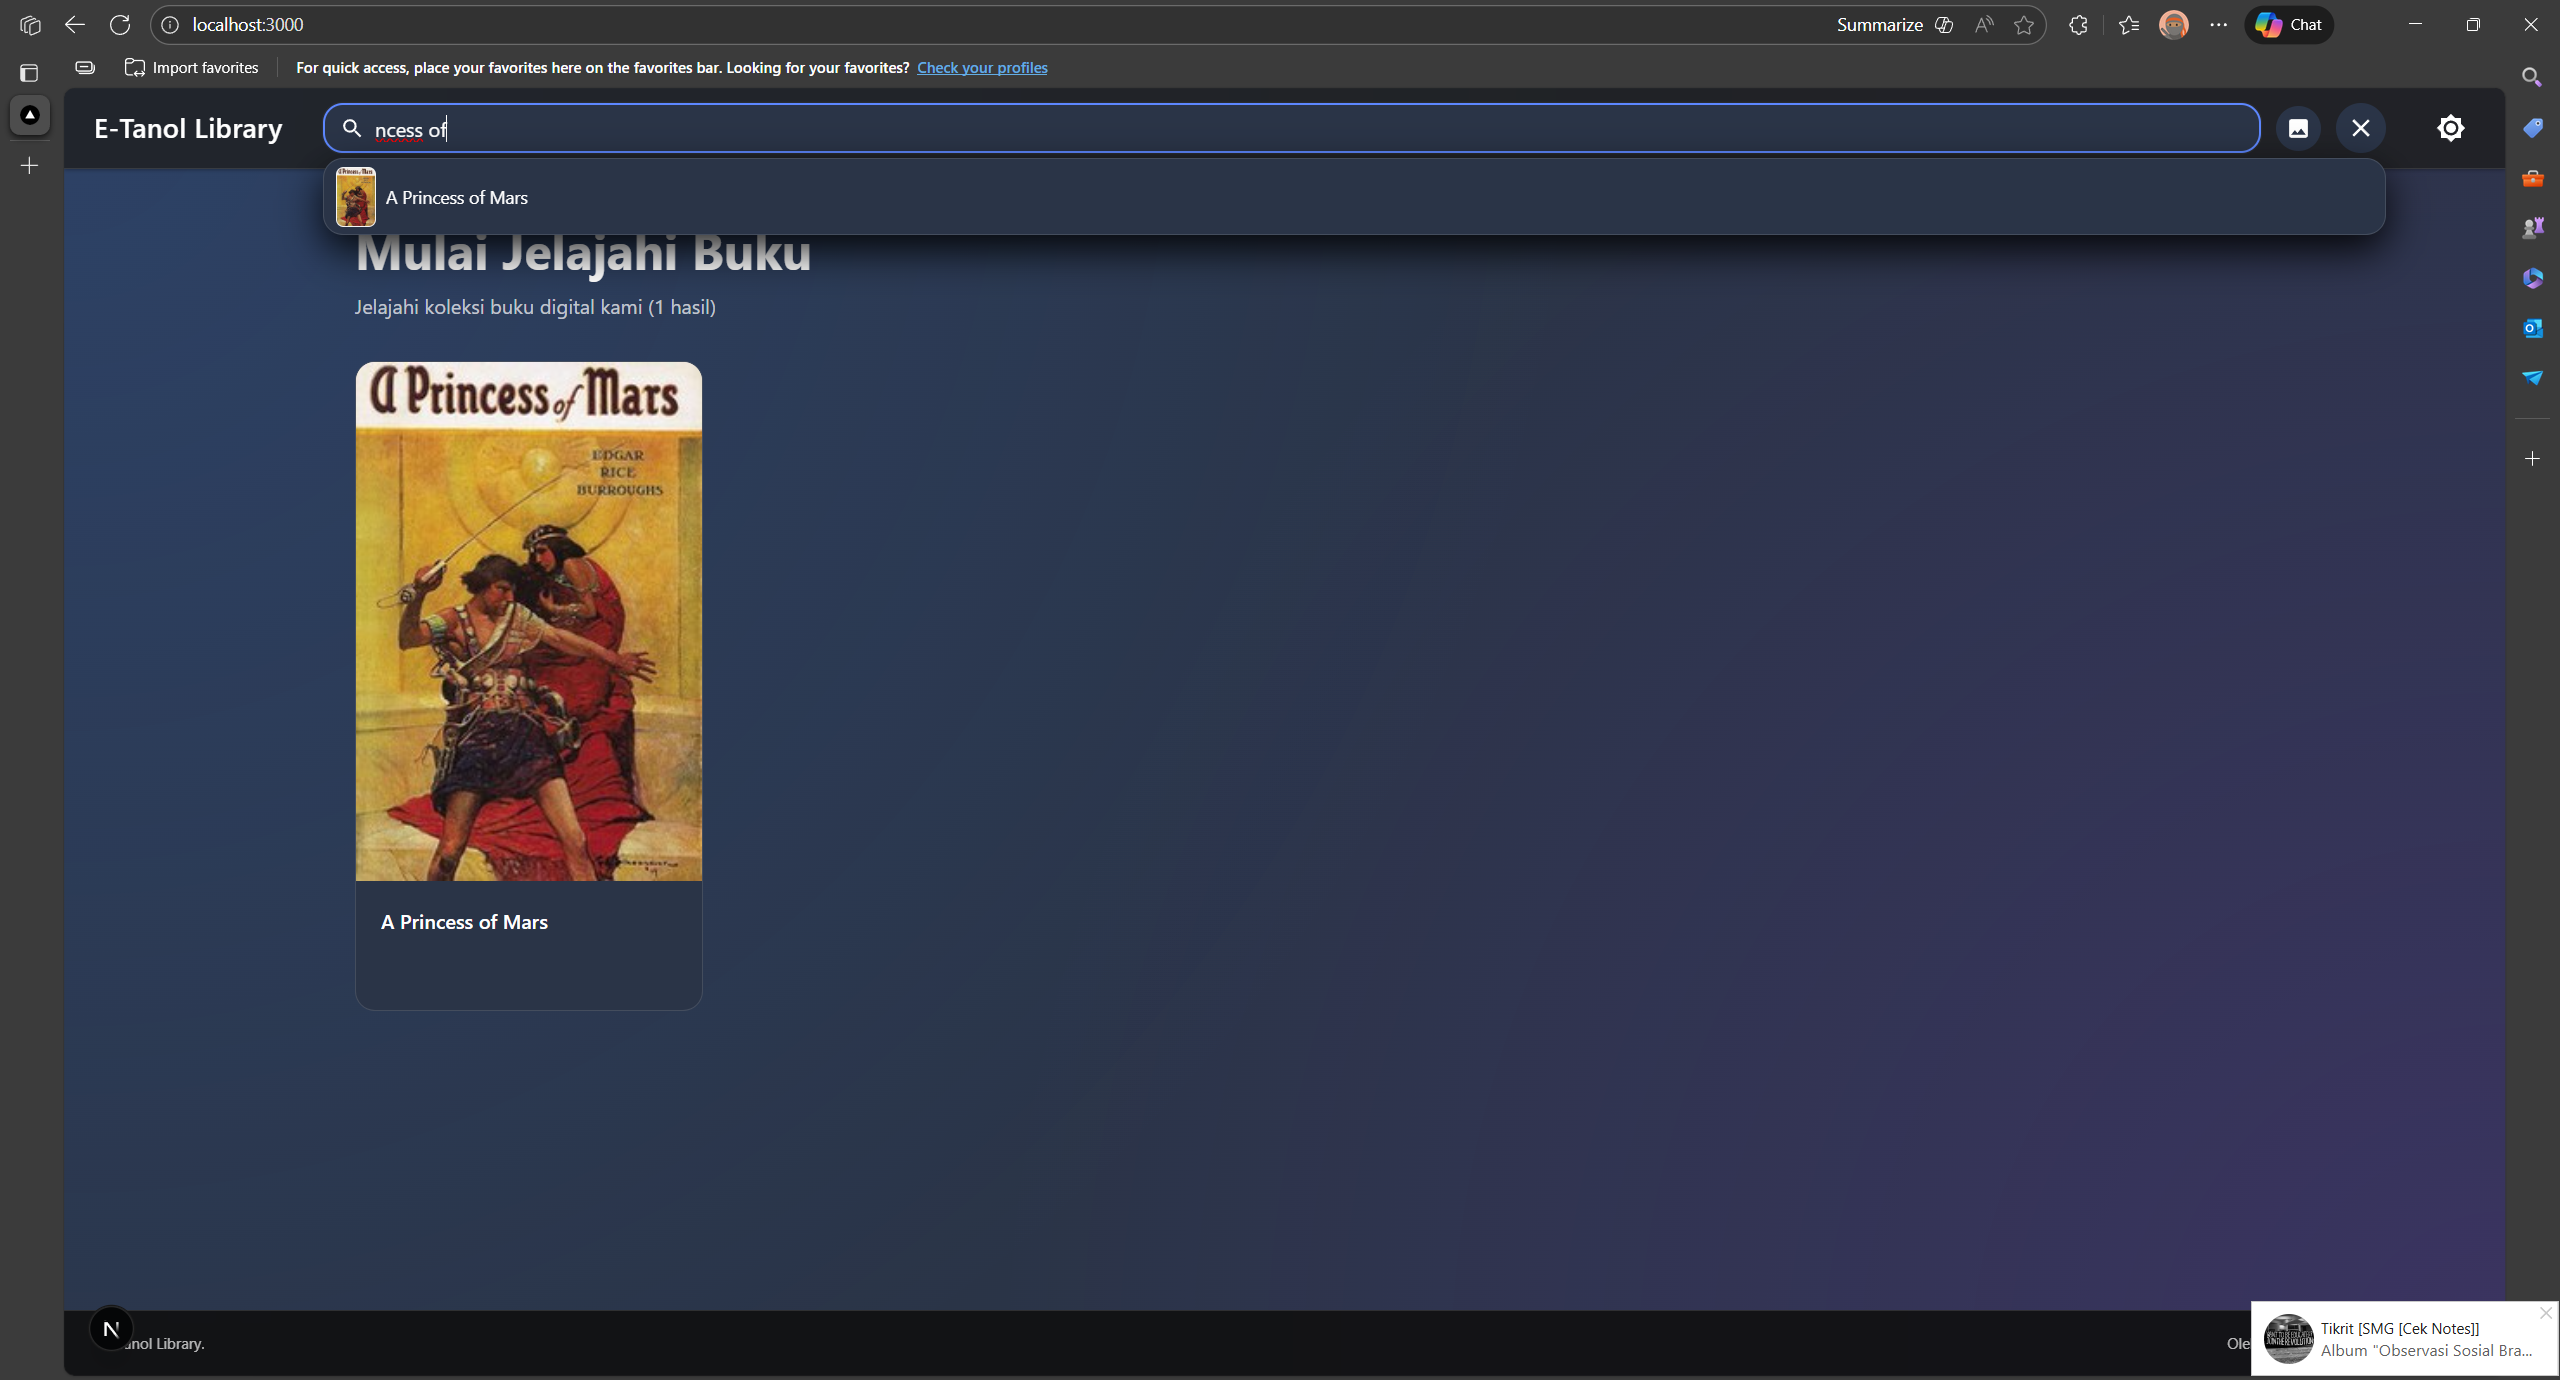
\includegraphics[width=0.75\textwidth]{img/eksperimen/judul/judul1.png}
    \caption{Tampilan hasil pencarian judul dengan katakunci "ncess of".}
    \label{fig:judul-1}
\end{figure}

\begin{figure}[H]
    \centering
    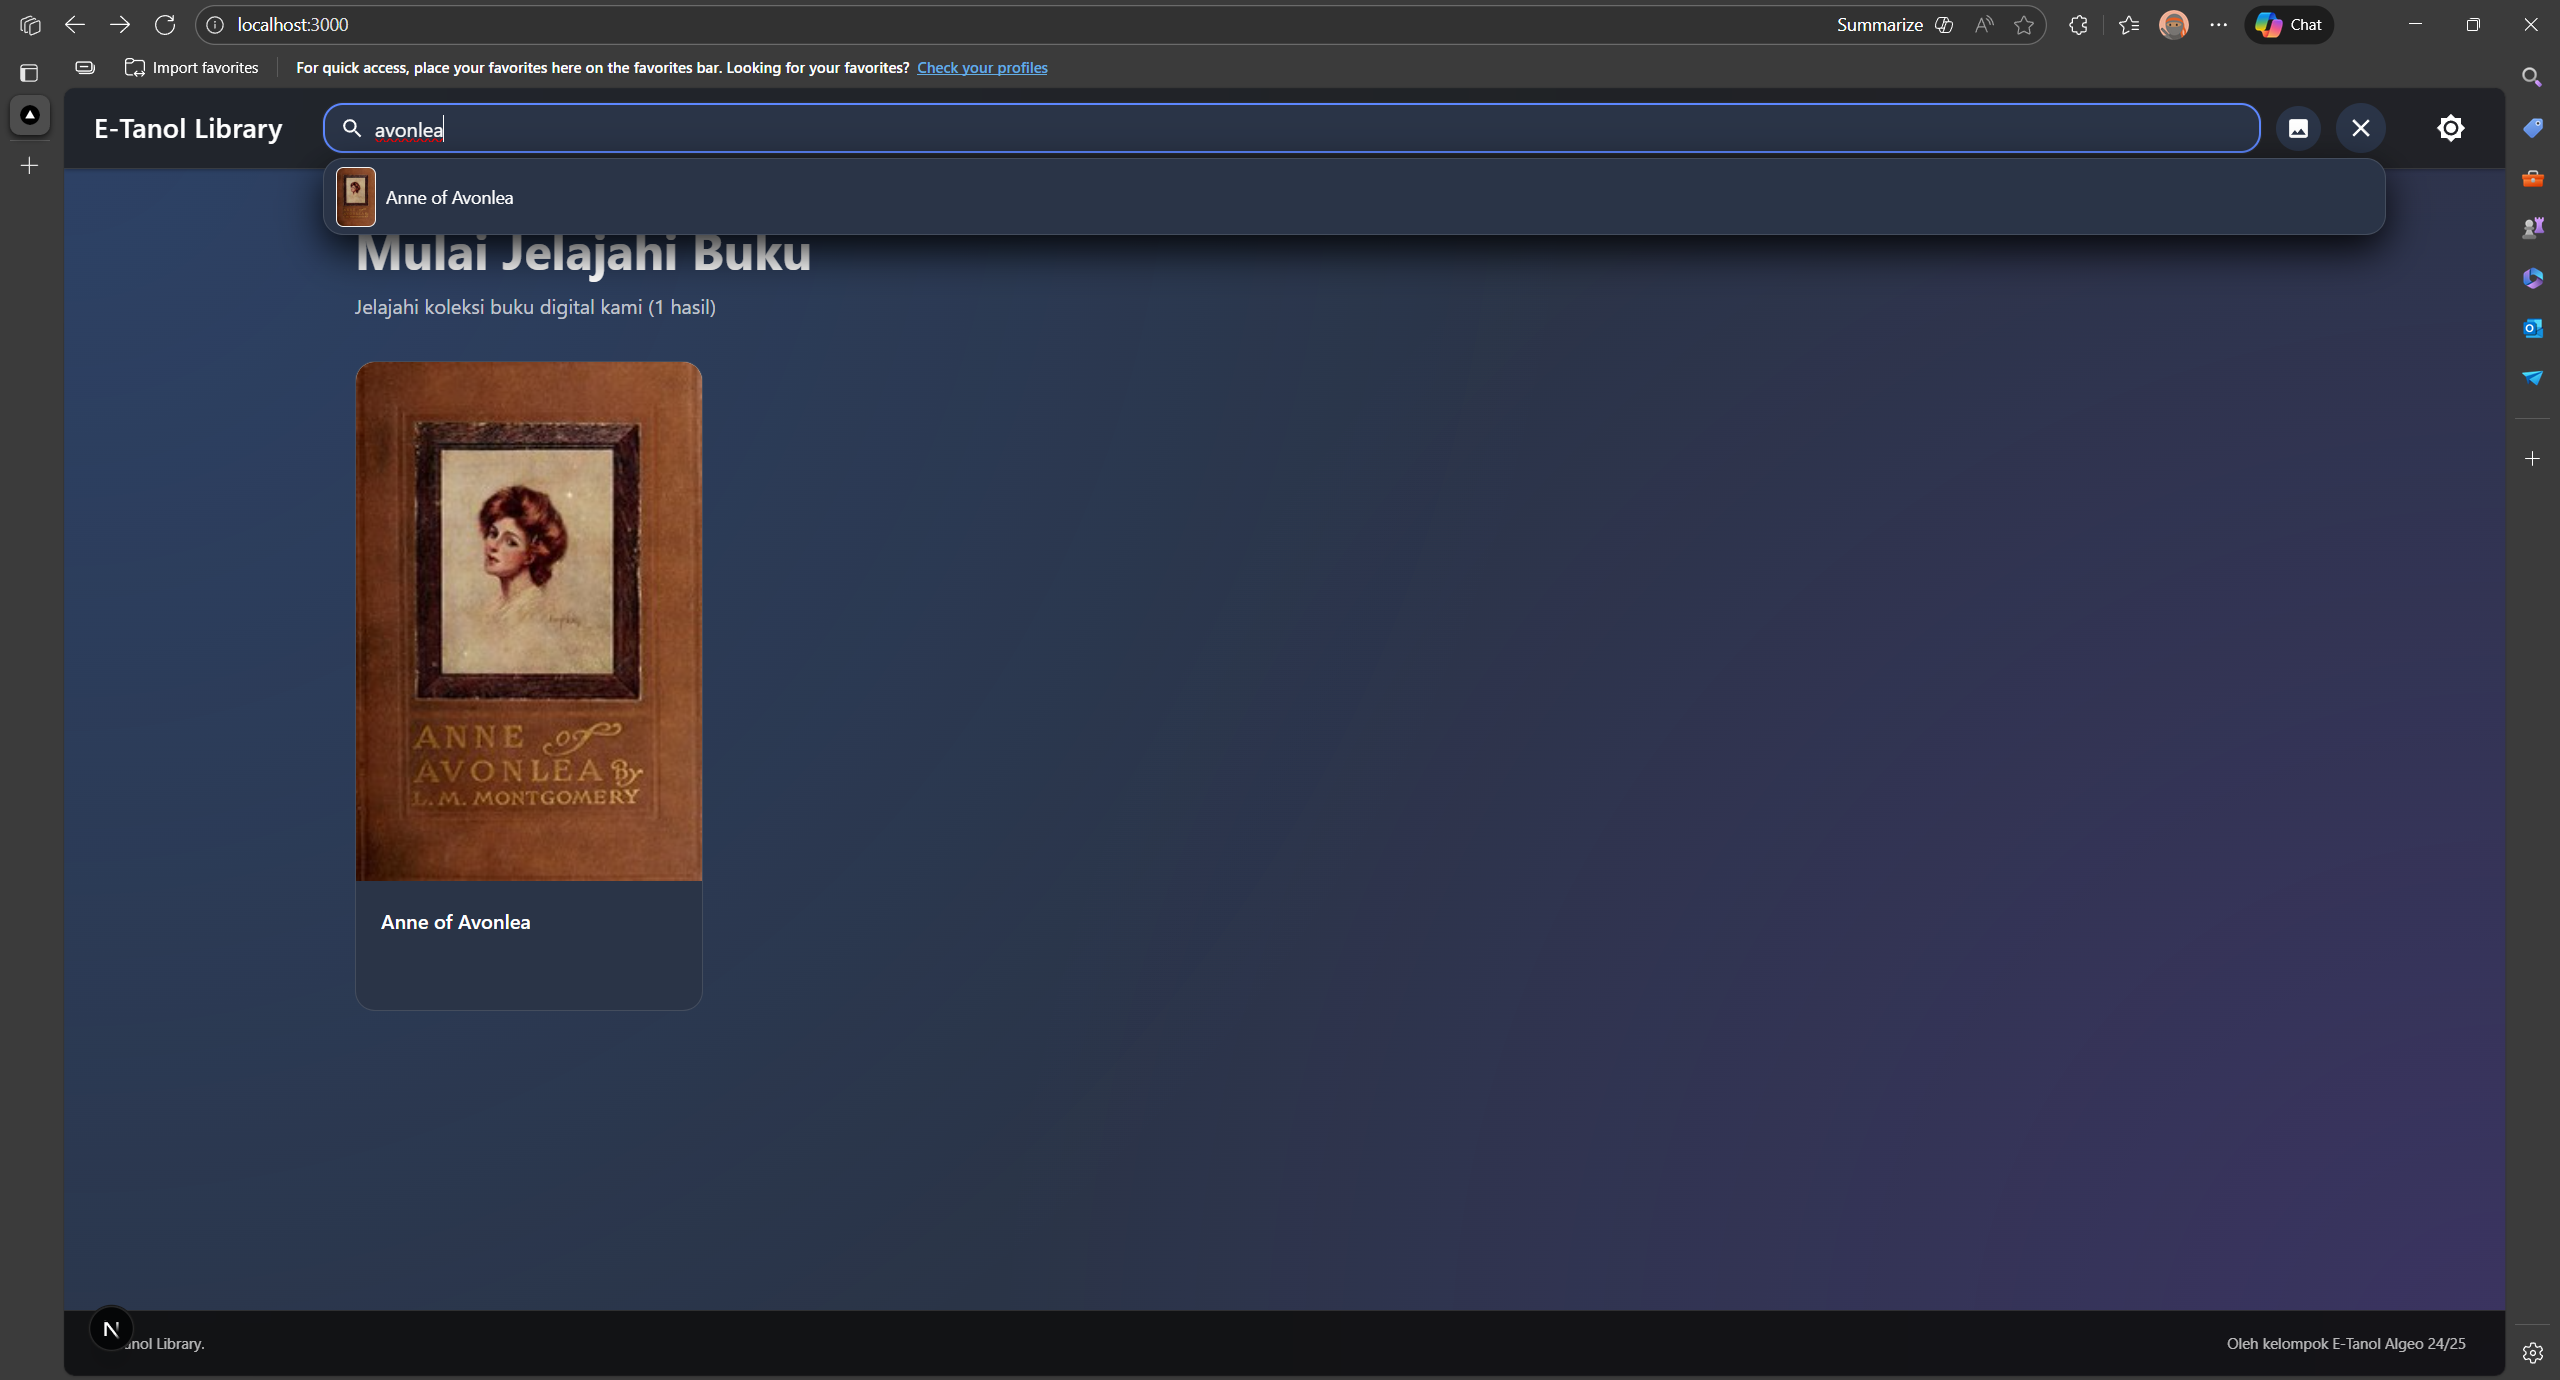
\includegraphics[width=0.75\textwidth]{img/eksperimen/judul/judul2.png}
    \caption{Tampilan hasil pencarian judul dengan katakunci "Avonlea".}
    \label{fig:judul-2}
\end{figure}

\begin{figure}[H]
    \centering
    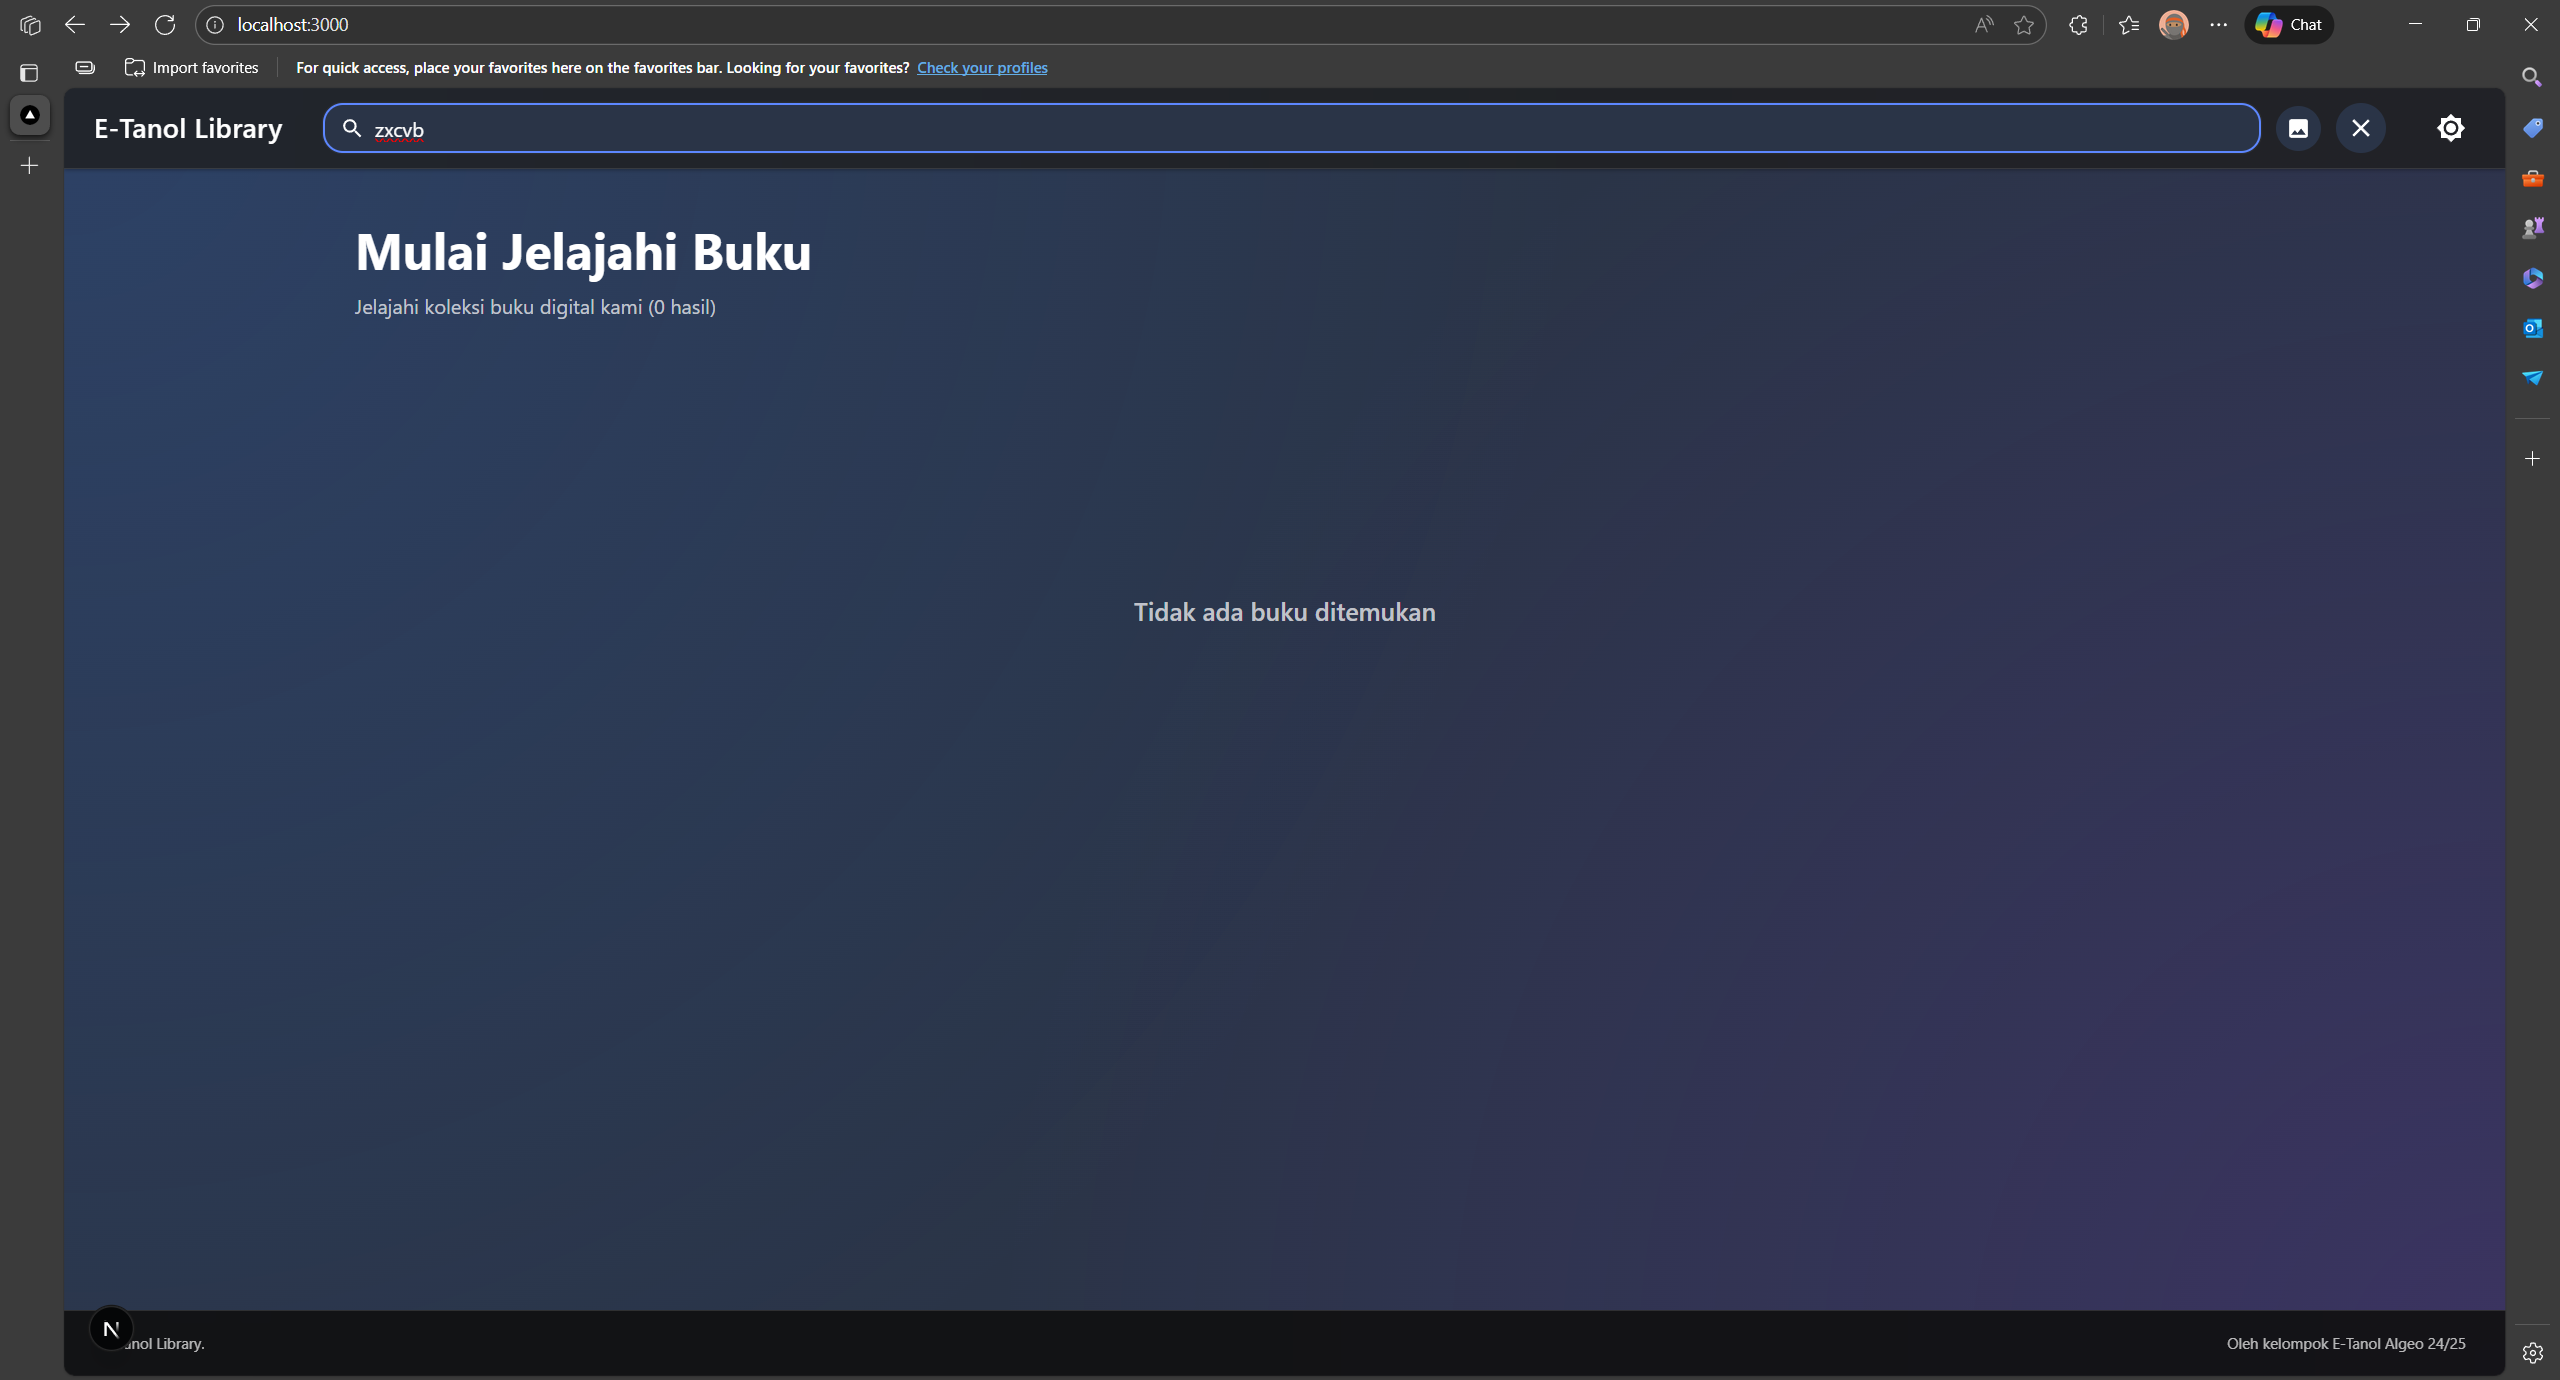
\includegraphics[width=0.75\textwidth]{img/eksperimen/judul/judul3.png}
    \caption{Tampilan hasil pencarian judul dengan katakunci "zxcvb".}
    \label{fig:judul-3}
\end{figure}

\textbf{Analisis Pencarian Judul (\textit{Substring Matching}):}
\begin{enumerate}[label=\textbf{\arabic*.}]
    \item \textbf{Validasi Pencocokan Pola Karakter (\textit{Pattern Matching})} \\
    Pada kasus uji pertama, input fragmentasi \texttt{"ncess of"} berhasil mengidentifikasi buku \textit{A Princess of Mars}. Hal ini membuktikan bahwa algoritma pencarian bekerja menggunakan metode \textit{substring matching} yang menyeluruh, di mana sistem tidak hanya mencari kecocokan pada awal kata (\textit{prefix}), tetapi mampu mendeteksi pola karakter yang berada di tengah maupun lintas-kata (\textit{cross-word boundary}).

    \item \textbf{Presisi Pencarian Kata Kunci} \\
    Kasus uji kedua dengan input \texttt{"Avonlea"} menunjukkan kemampuan sistem dalam melakukan filtrasi data yang presisi. Sistem berhasil mengisolasi buku \textit{Anne of Avonlea} dari sekian banyak koleksi, memverifikasi bahwa fungsi pencarian utama berjalan sesuai spesifikasi fungsional untuk pengambilan informasi (\textit{information retrieval}) dasar.

    \item \textbf{Penanganan Hasil Kosong (Empty State Handling)} \\
    Pengujian ketiga menggunakan input string acak \texttt{"zxcvb"} menunjukkan respons sistem yang valid. Sistem tidak mengalami kegagalan (\textit{crash}) melainkan memberikan umpan balik visual berupa pesan \texttt{"Tidak ada buku ditemukan"}. Ini menunjukkan adanya mekanisme \textit{conditional rendering} yang baik pada antarmuka pengguna untuk menangani kondisi ketika kueri tidak menghasilkan kecocokan dalam basis data.
\end{enumerate}

\subsubsection{Pencarian Buku Berdasarkan Gambar Sampul (Asisten \& Mandiri)}
Pengujian ini mengevaluasi kinerja \textit{Image Similarity} berbasis PCA dengan penggunaan threshold 0.3. Semakin kecil skor semakin mirip.

\begin{table}[H]
    \centering
    \begin{tabularx}{\linewidth}{c X X X c X}
        \toprule
        \textbf{No} & \textbf{Sumber Gambar} & \textbf{Kondisi} & \textbf{Target Buku} & \textbf{Skor Kemiripan} & \textbf{Hasil Sistem} \\
        \midrule
        1 & Dataset Asisten & Sedikit Buram & The Wonderful Wizard of Oz & 0.01 & Top 1: The Wonderful Wizard of Oz \\
        2 & Dataset Asisten & Teks Judul Tidak Jelas & A Treatise of Human Nature & 0.2 & Top 1: A Treatise of Human Nature \\
        3 & Dataset Asisten & Warna Lebih Terang & The Adventures of Sherlock Holmes & 0.06 & Top 1: The Adventures of Sherlock Holmes \\
        4 & Internet & Sedikit Buram & The Return of Sherlock Holmes & 0 & Top 1: The Return of Sherlock Holmes \\
        5 & Internet & Warna Lebih Terang & A Princess of Mars & 0 & Top 1: A Princess of Mars \\
        \bottomrule
    \end{tabularx}
    \caption{Hasil Pengujian Pencarian Buku Berdasarkan Gambar Sampul}
    \label{tab:hasil-pencarian-gambar}
\end{table}

\begin{figure}[H]
    \centering
    \begin{minipage}{0.35\textwidth}
        \centering
        
\includegraphics[width=\linewidth]{img/eksperimen/image/imageTC1.png}
        \caption{Image Test Case 1}
        \label{fig:image-tc-1}
    \end{minipage}
    \hfill
    \begin{minipage}{0.60\textwidth}
        \centering
        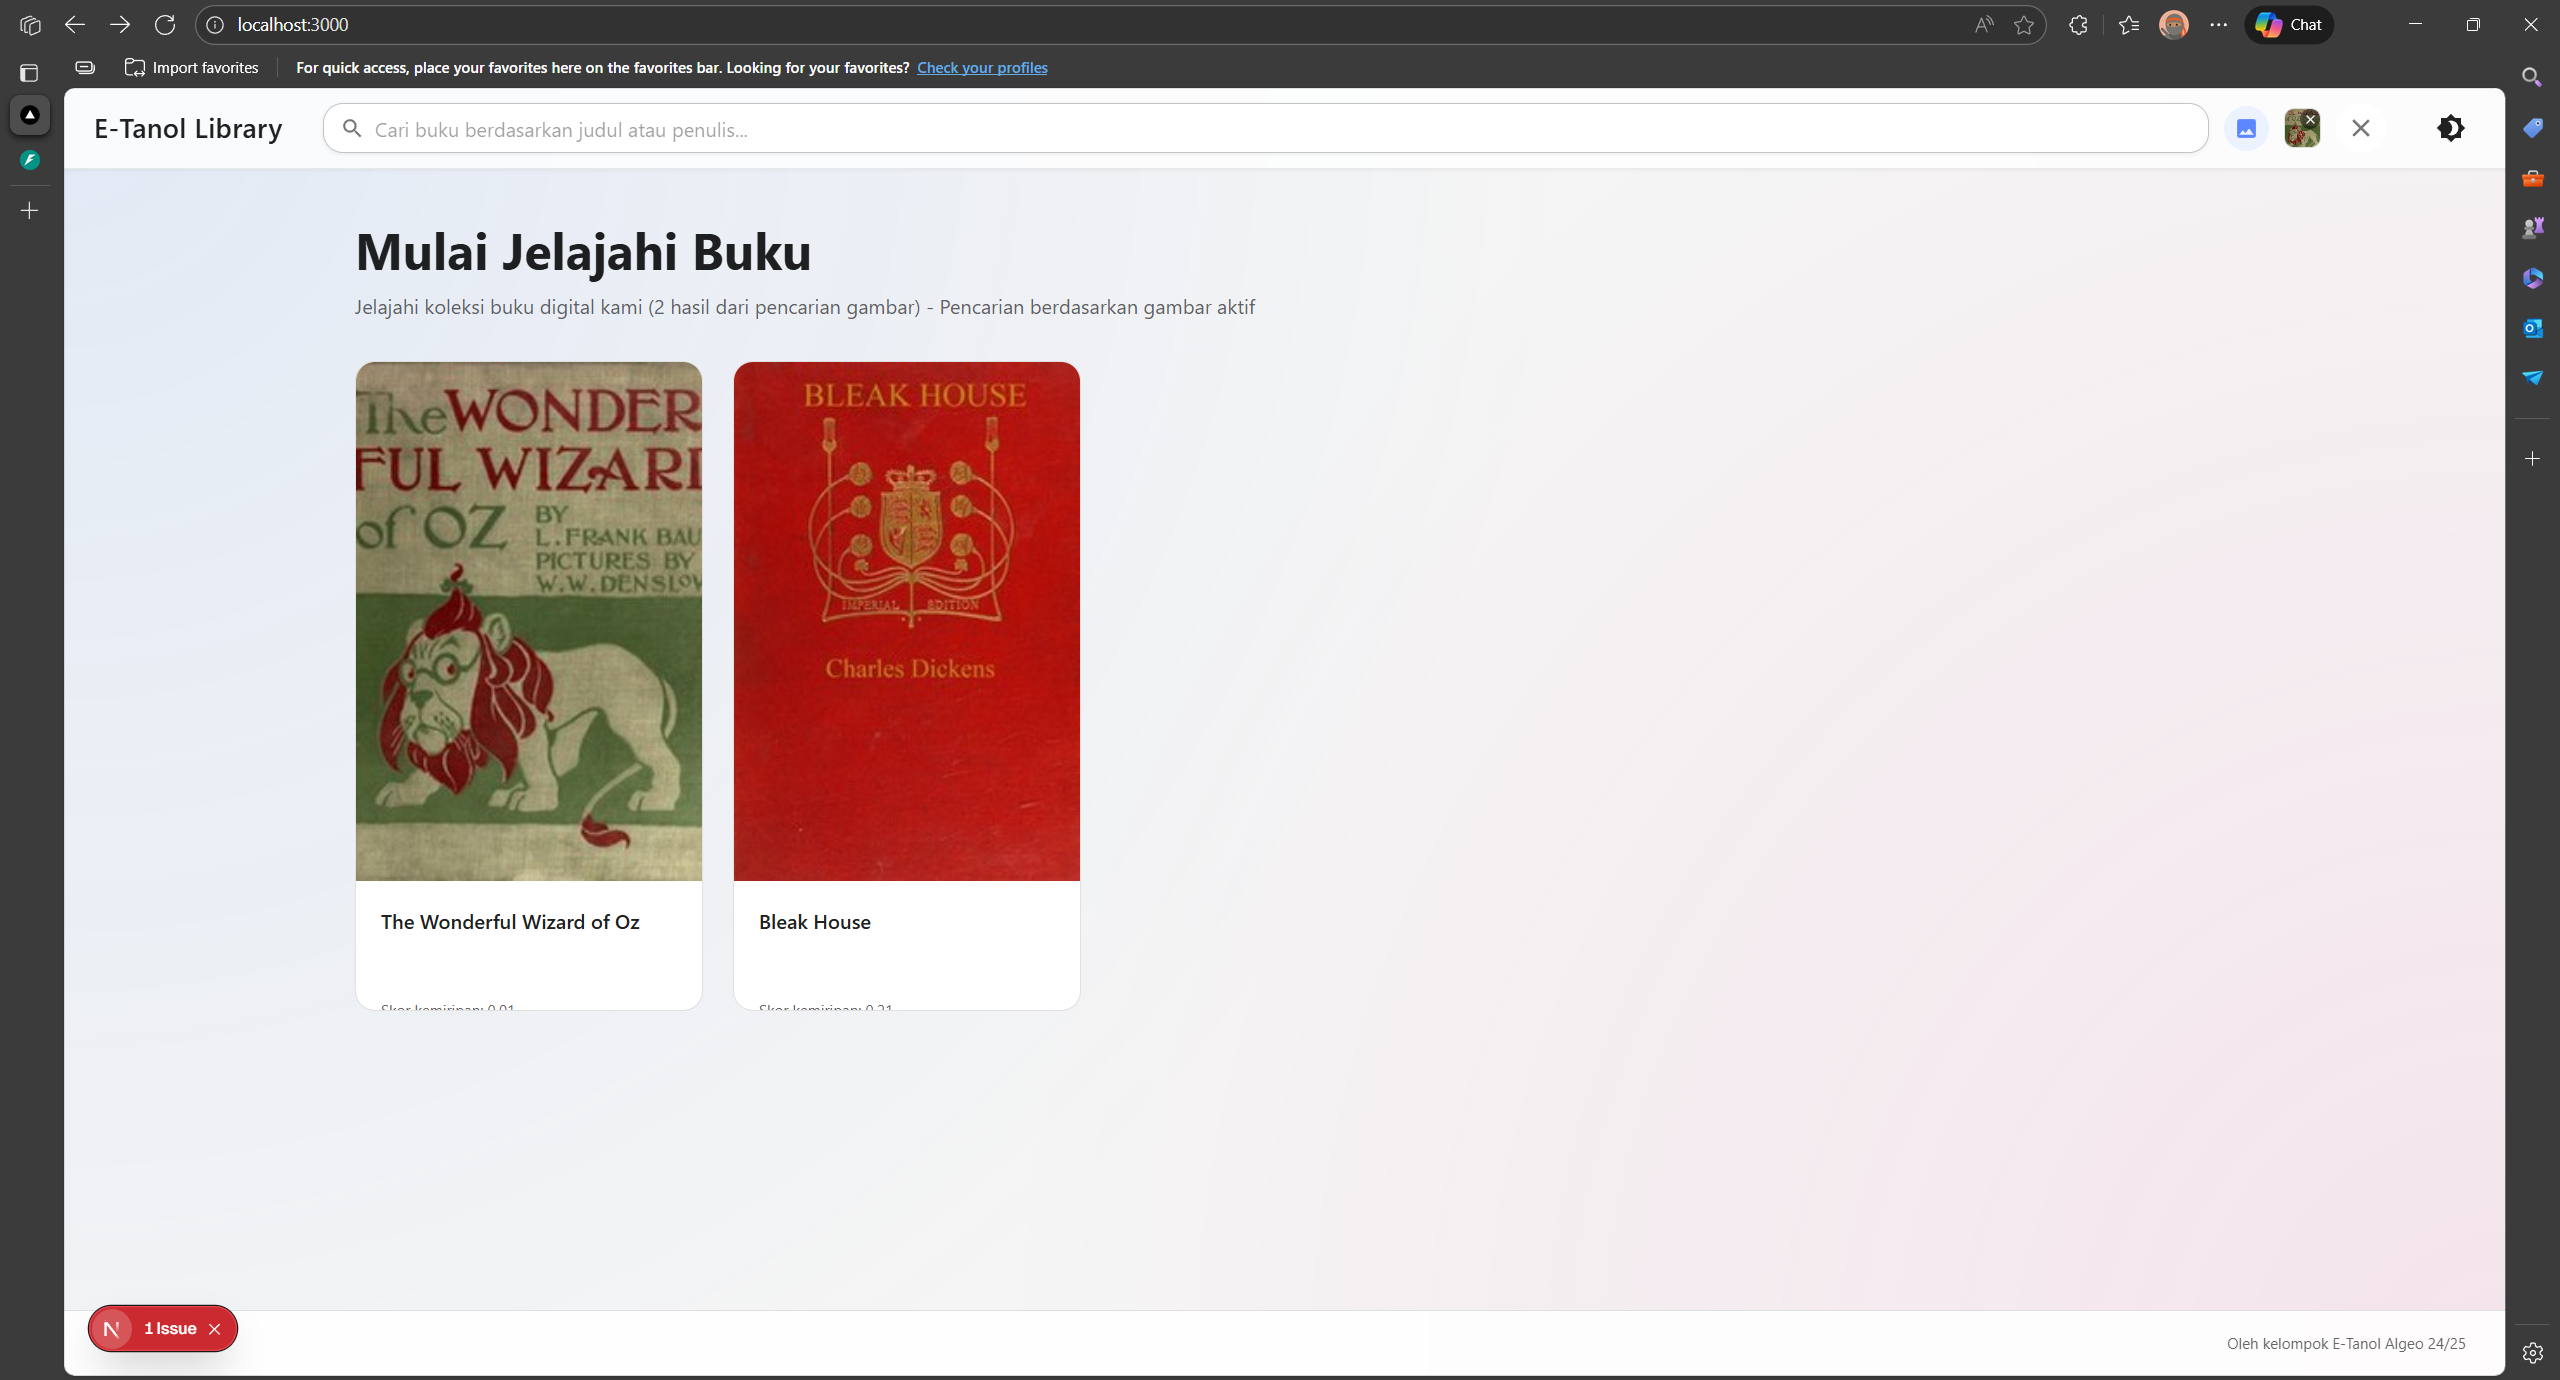
\includegraphics[width=\linewidth]{img/eksperimen/image/result/imageTC1-result.png}
        \caption{Hasil Pencarian Image Test Case 1}
        \label{fig:image-tc-1-res}
    \end{minipage}
\end{figure}

\begin{figure}[H]
    \centering
    \begin{minipage}{0.35\textwidth}
        \centering
        
\includegraphics[width=\linewidth]{img/eksperimen/image/imageTC2.png}
        \caption{Image Test Case 2}
        \label{fig:image-tc-2}
    \end{minipage}
    \hfill
    \begin{minipage}{0.60\textwidth}
        \centering
        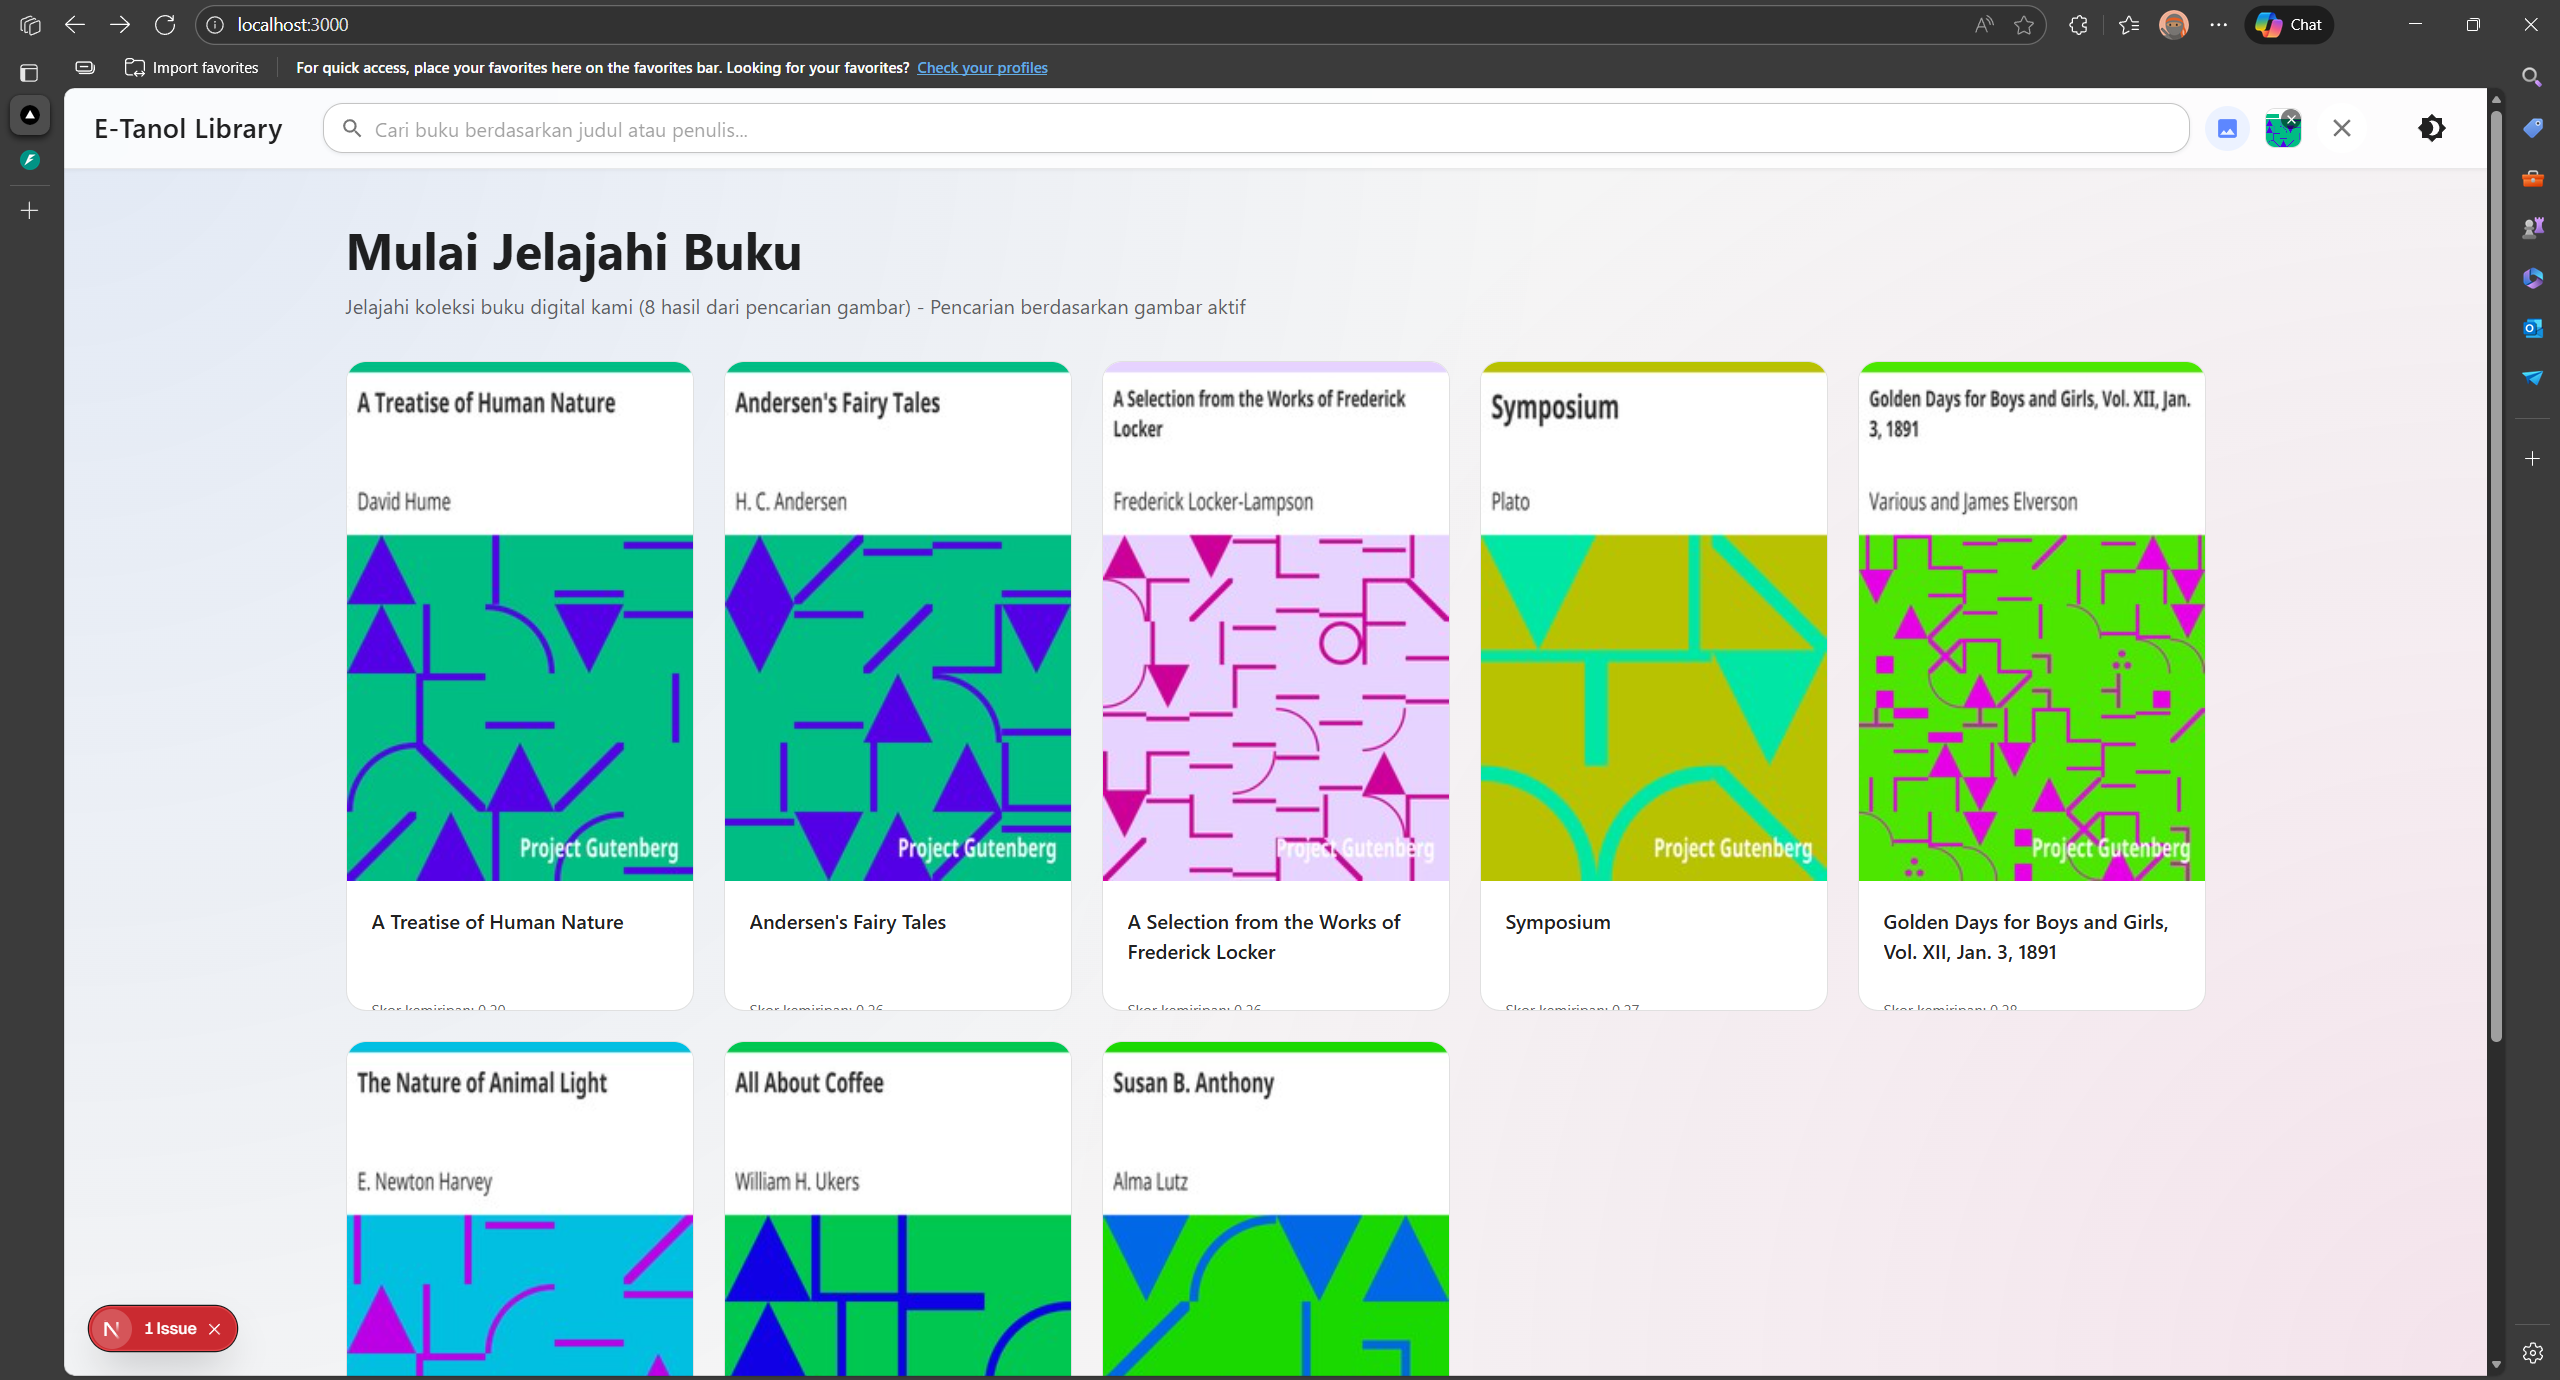
\includegraphics[width=\linewidth]{img/eksperimen/image/result/imageTC2-result.png}
        \caption{Hasil Pencarian Image Test Case 2}
        \label{fig:image-tc-2-res}
    \end{minipage}
\end{figure}

\begin{figure}[H]
    \centering
    \begin{minipage}{0.35\textwidth}
        \centering
        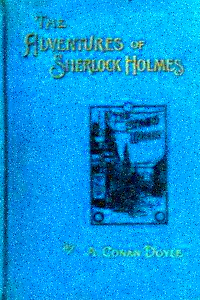
\includegraphics[width=\linewidth]{img/eksperimen/image/imageTC3.png}
        \caption{Image Test Case 3}
        \label{fig:image-tc-3}
    \end{minipage}
    \hfill
    \begin{minipage}{0.60\textwidth}
        \centering
        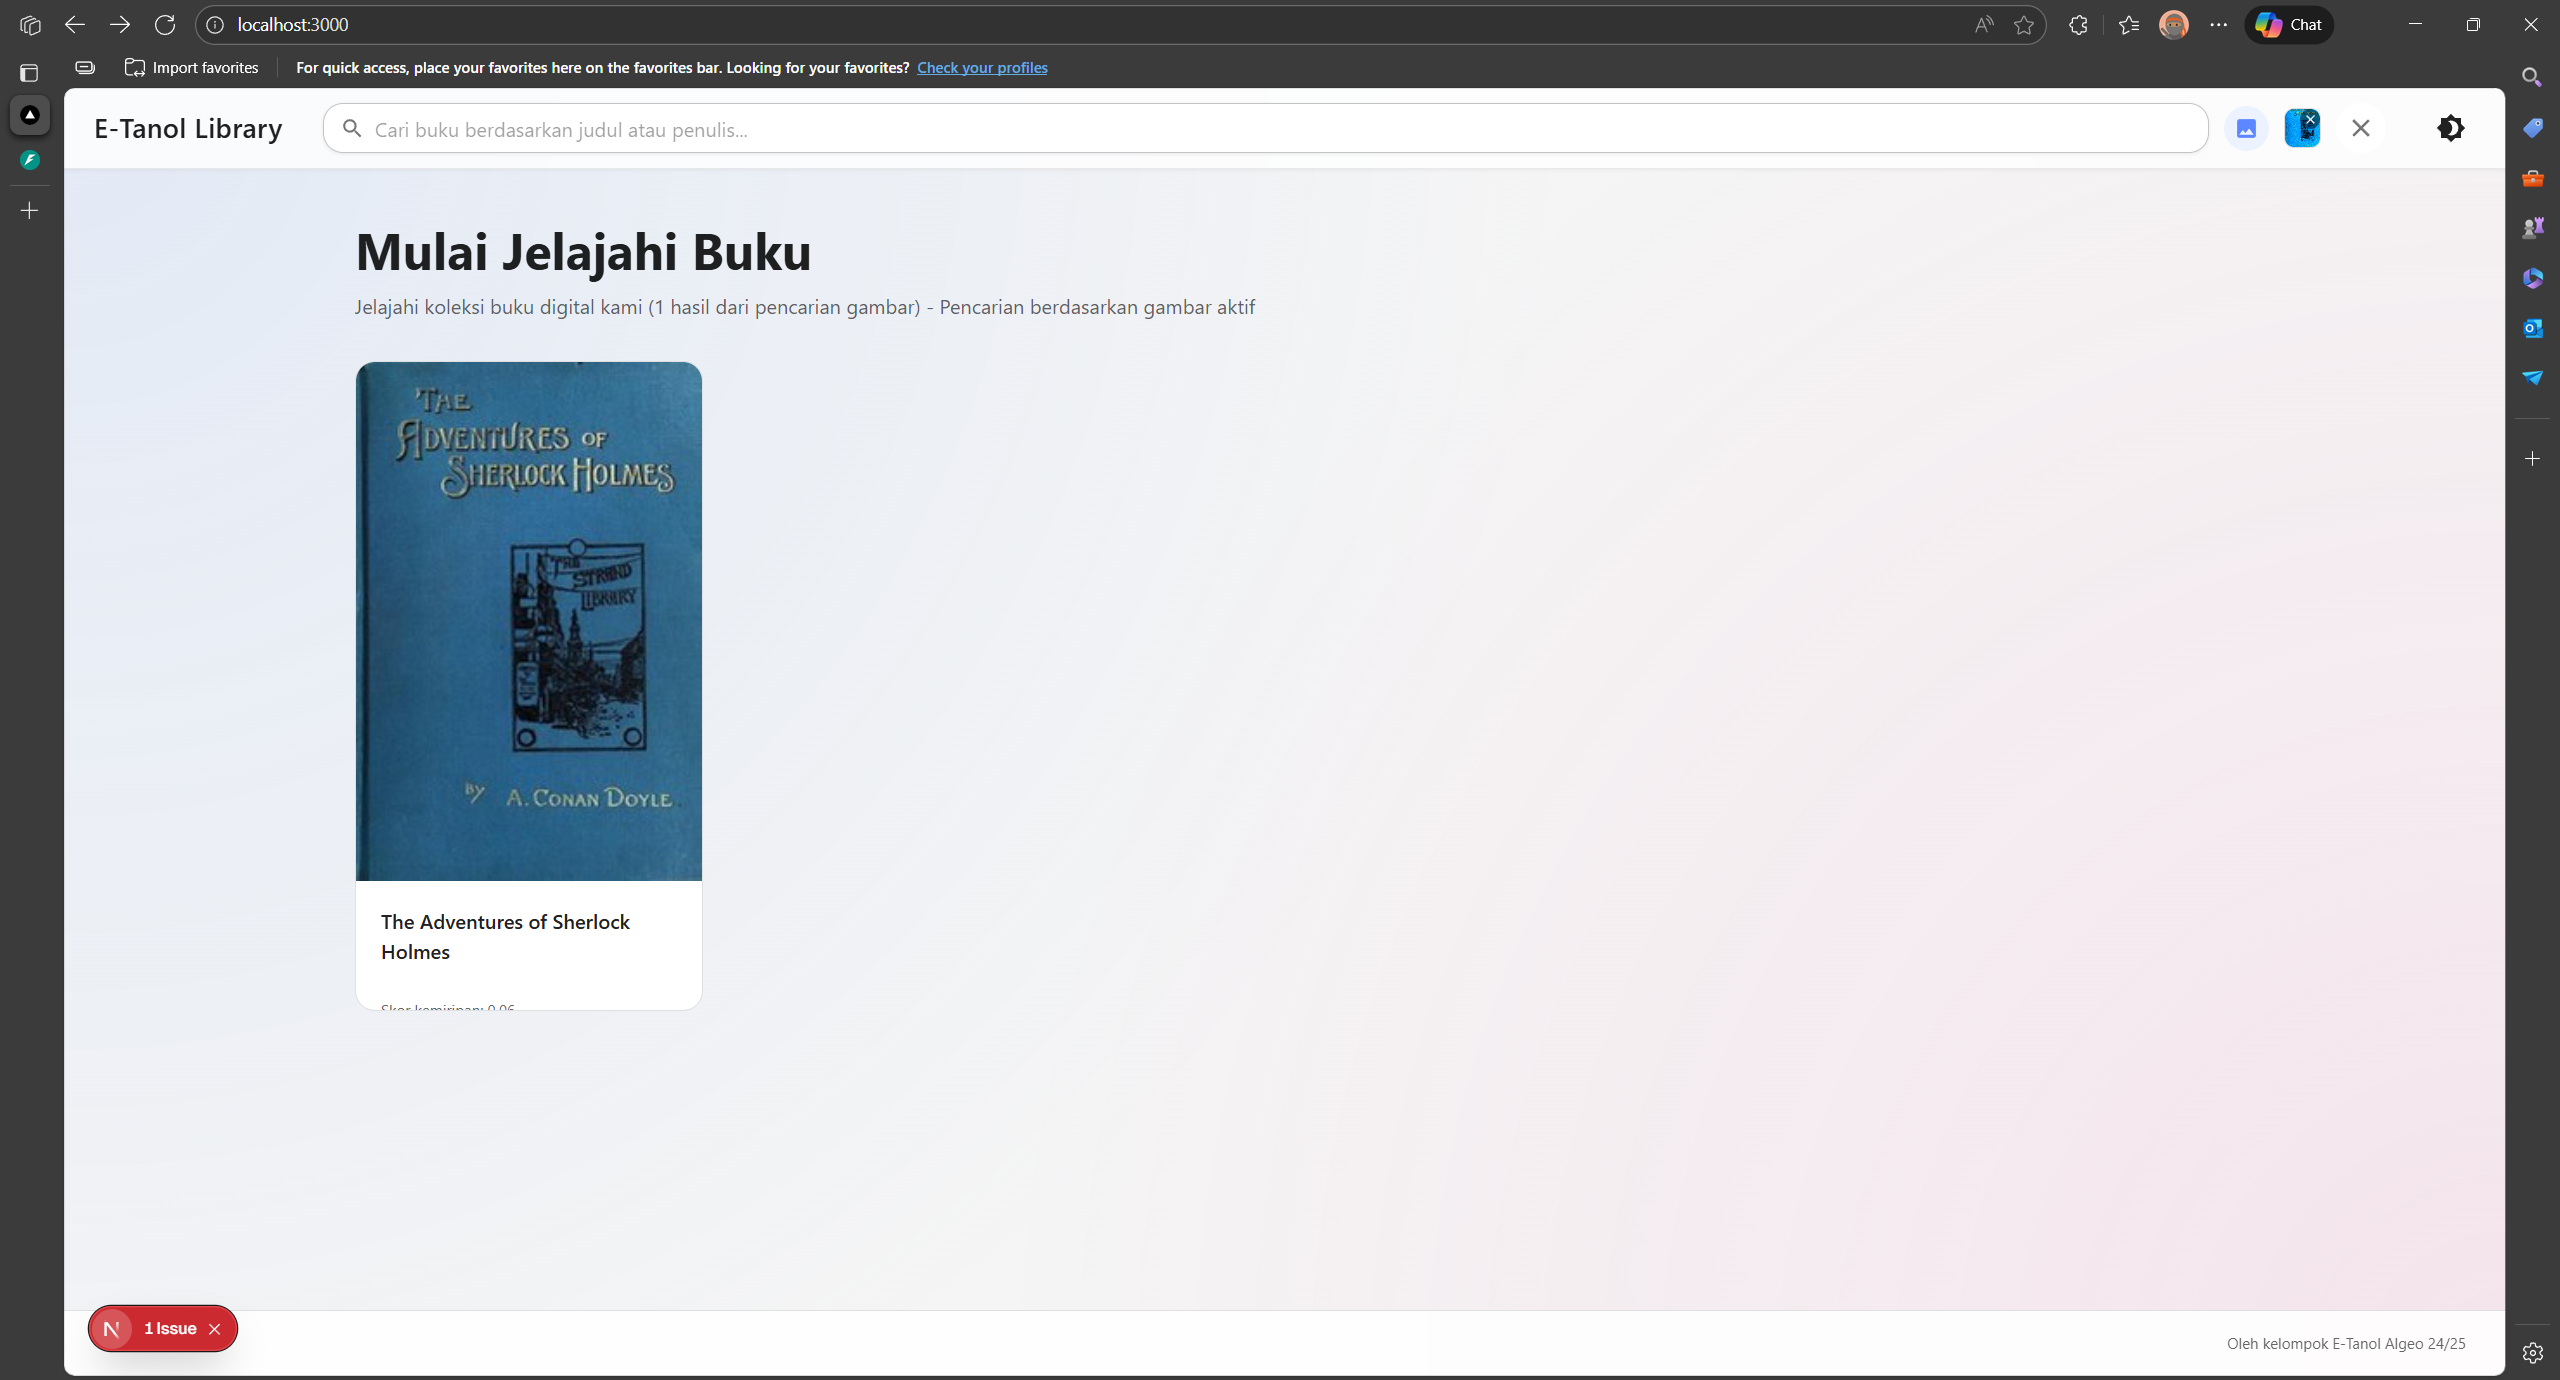
\includegraphics[width=\linewidth]{img/eksperimen/image/result/imageTC3-result.png}
        \caption{Hasil Pencarian Image Test Case 3}
        \label{fig:image-tc-3-res}
    \end{minipage}
\end{figure}

\begin{figure}[H]
    \centering
    \begin{minipage}{0.35\textwidth}
        \centering
        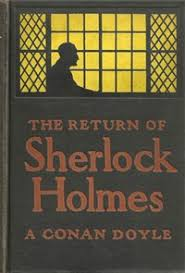
\includegraphics[width=\linewidth]{img/eksperimen/image/imageM1.jpeg}
        \caption{Image Mandiri 1}
        \label{fig:image-m-1}
    \end{minipage}
    \hfill
    \begin{minipage}{0.60\textwidth}
        \centering
        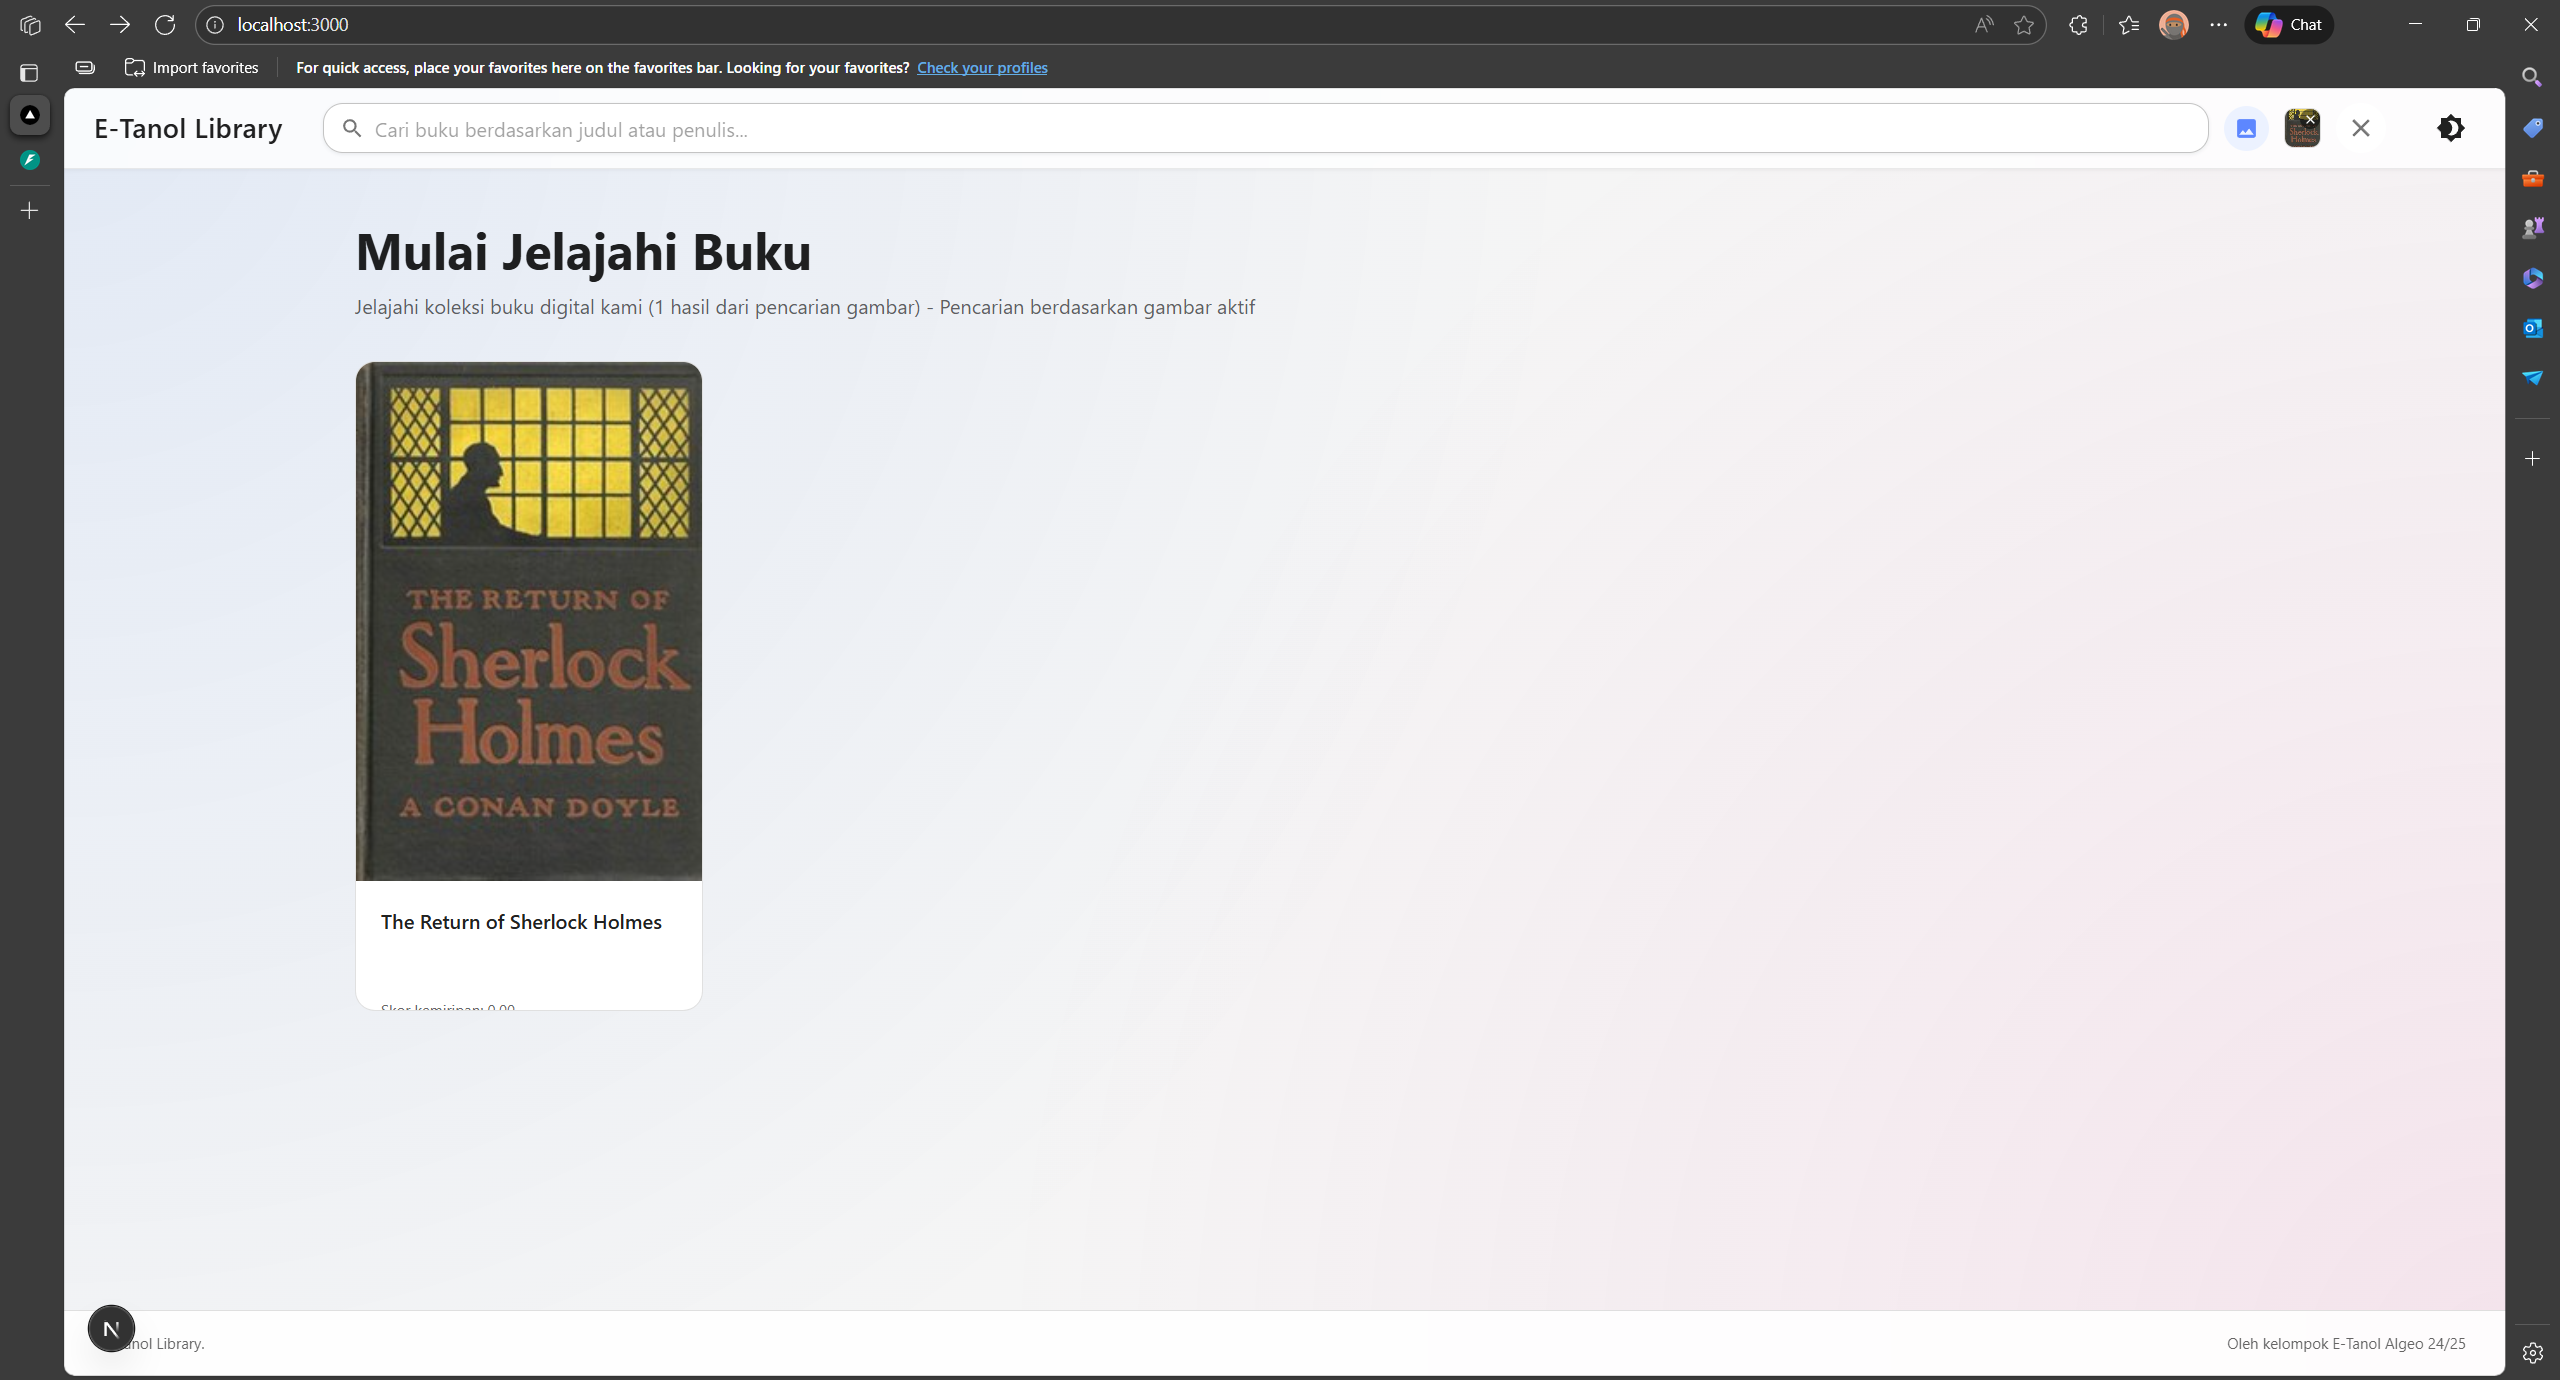
\includegraphics[width=\linewidth]{img/eksperimen/image/result/imageM1-result.png}
        \caption{Hasil Pencarian Image Mandiri 1}
        \label{fig:image-m-1-res}
    \end{minipage}
\end{figure}

\begin{figure}[H]
    \centering
    \begin{minipage}{0.35\textwidth}
        \centering
        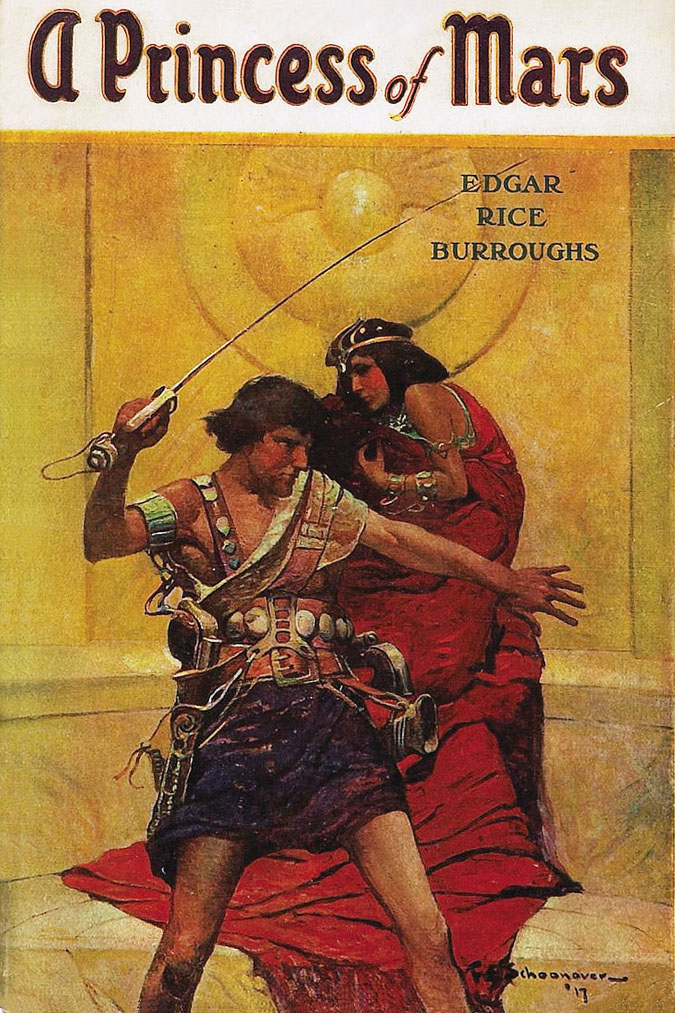
\includegraphics[width=\linewidth]{img/eksperimen/image/imageM2.jpg}
        \caption{Image Mandiri 2}
        \label{fig:image-m-2}
    \end{minipage}
    \hfill
    \begin{minipage}{0.60\textwidth}
        \centering
        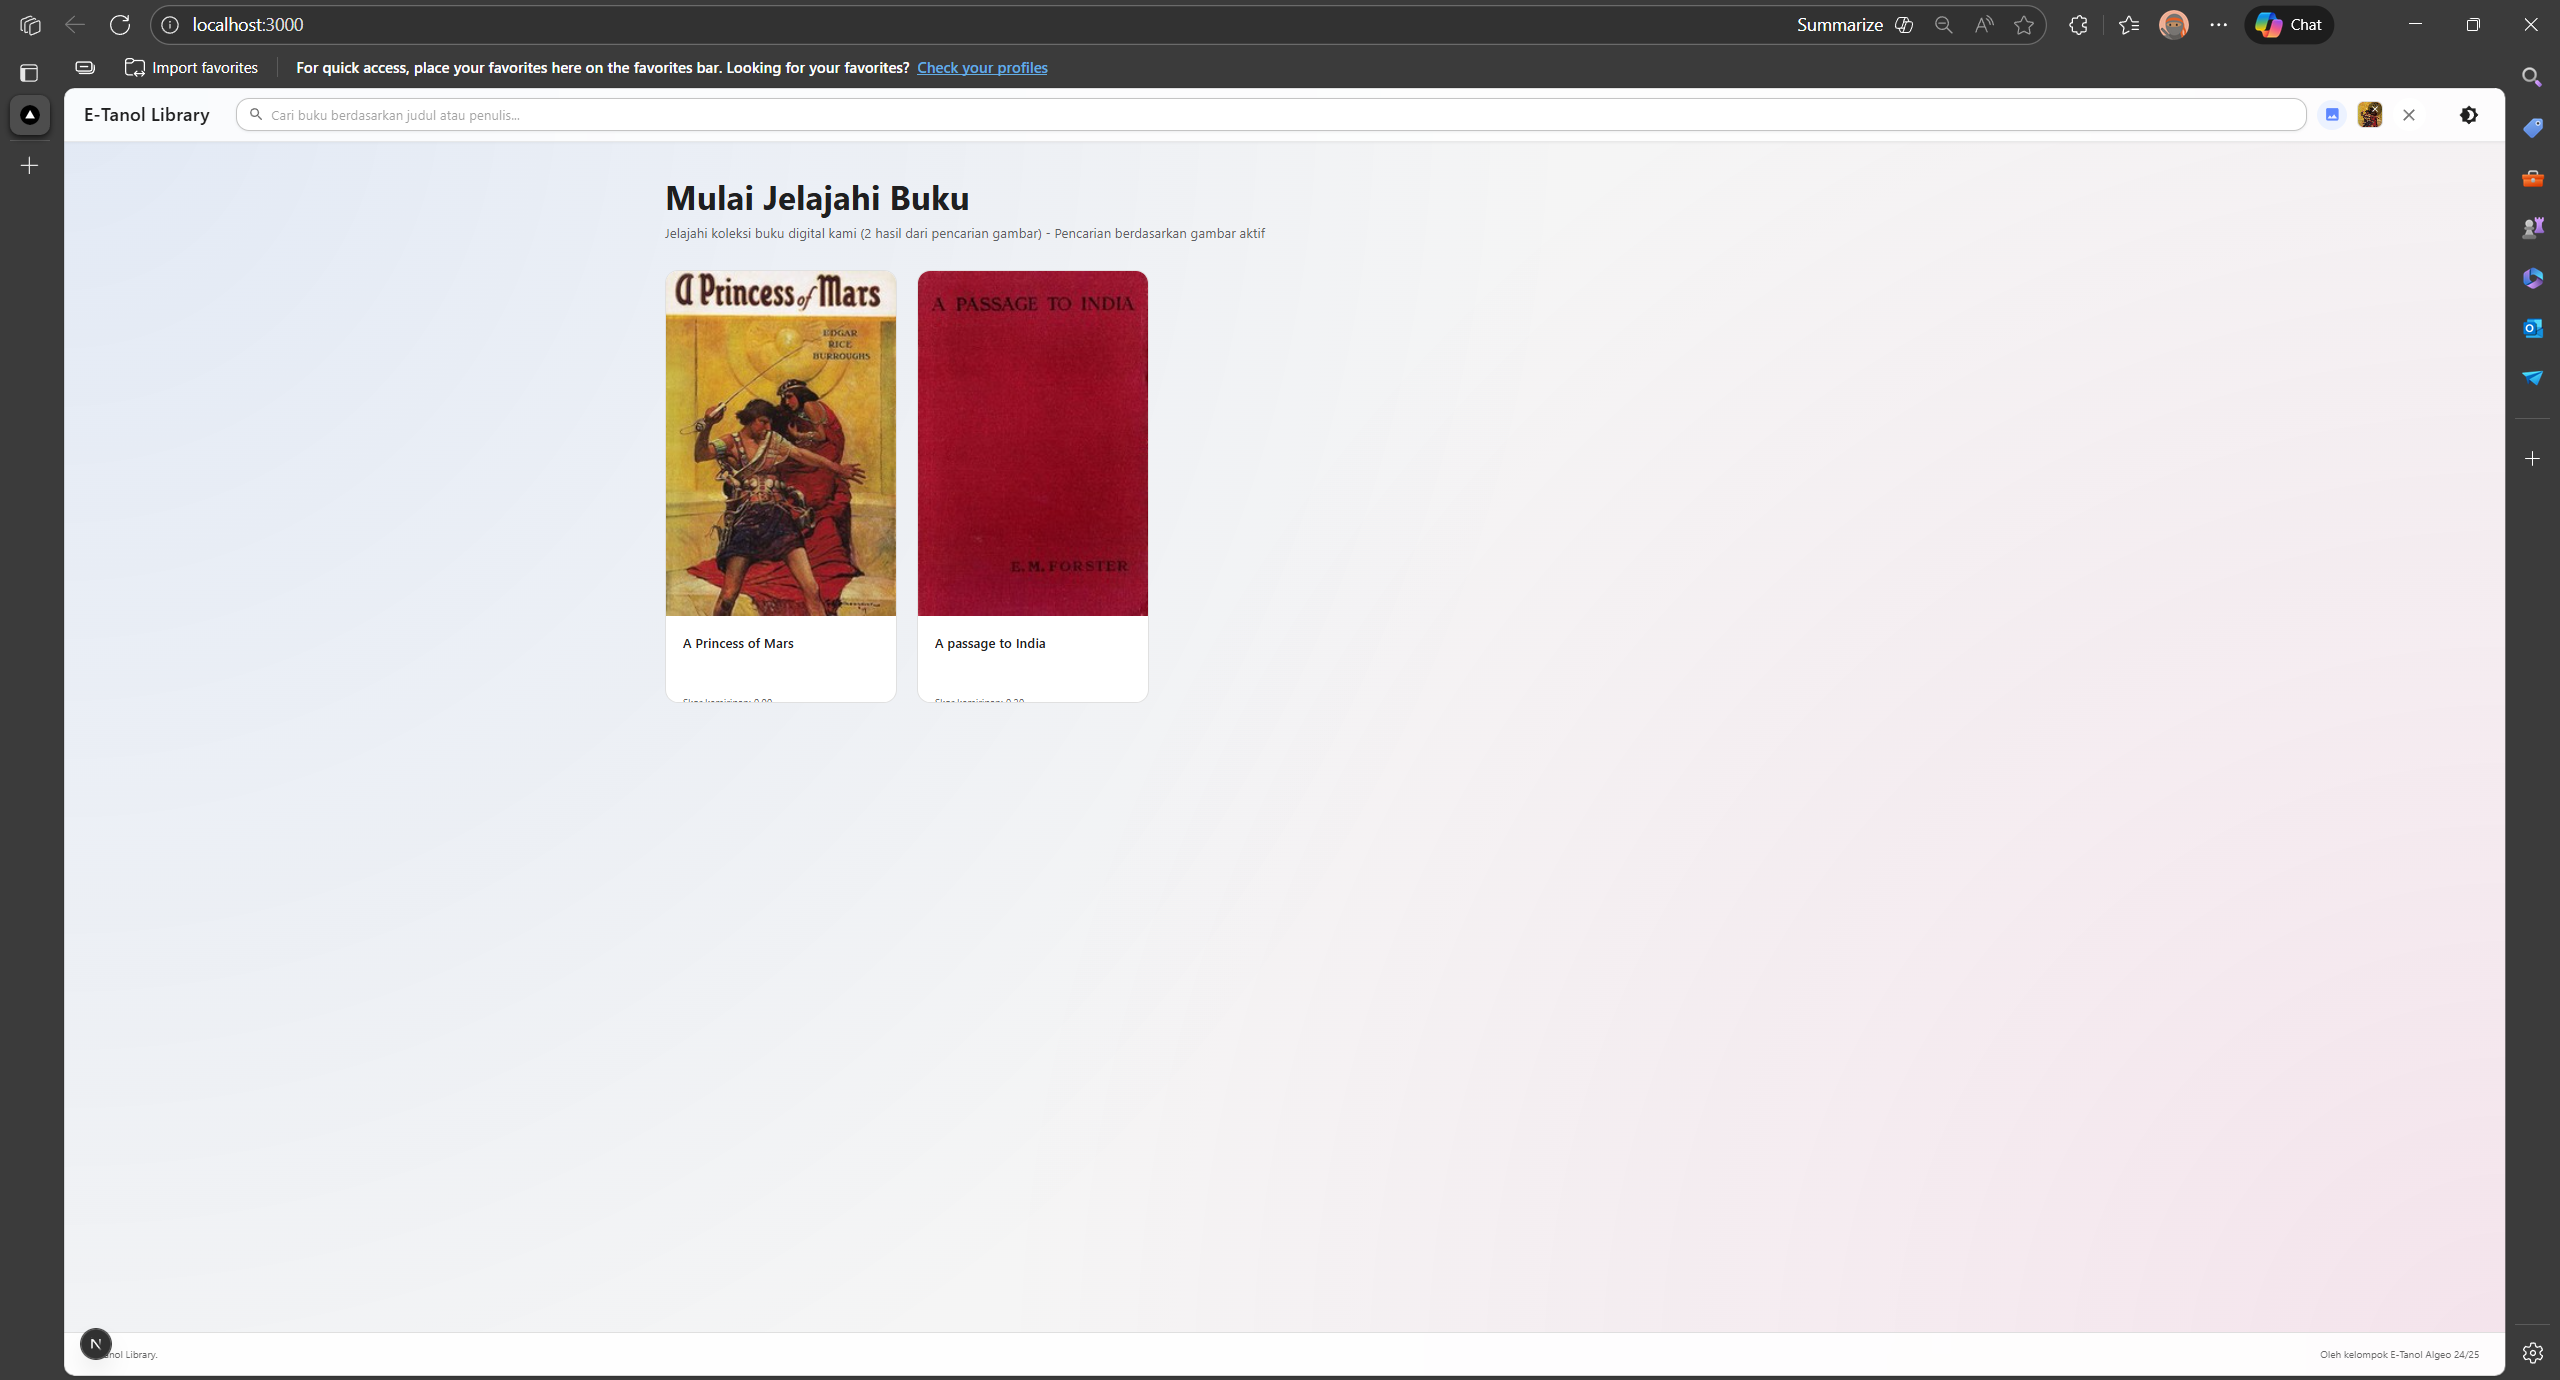
\includegraphics[width=\linewidth]{img/eksperimen/image/result/imageM2-result.png}
        \caption{Hasil Pencarian Image Mandiri 2}
        \label{fig:image-m-2-res}
    \end{minipage}
\end{figure}

\textbf{Analisis Pencarian Gambar (PCA/Eigenface):}
\begin{enumerate}[label=\textbf{\arabic*.}]
    \item \textbf{Akurasi pada Dataset Asisten} \\
    Sistem menunjukkan performa yang sangat baik pada data uji standar. Meskipun terdapat gangguan (\textit{noise}) berupa efek buram atau teks yang tidak jelas (Kasus 1 dan 2), sistem tetap mampu mengenali buku dengan nilai \textit{Cosine Distance} yang rendah (mendekati 0). Hal ini mengindikasikan bahwa fitur utama (\textit{principal components}) yang diekstrak oleh PCA cukup \textit{robust} terhadap degradasi kualitas citra minor, karena pengukuran berbasis sudut vektor lebih memprioritaskan kesamaan struktur visual (pola) daripada intensitas piksel absolut.

    \item \textbf{Ketahanan terhadap Variasi Pencahayaan} \\
    Pada kasus uji ke-3 dan ke-5, perubahan intensitas cahaya (lebih terang) tidak menggagalkan proses identifikasi. Normalisasi vektor citra dan pemusatan data (\textit{mean centering}) pada tahap preprocessing berperan penting dalam meminimalisir dampak perbedaan pencahayaan global.

    \item \textbf{Identifikasi Citra Identik} \\
    Pada Kasus 4 dan 5 (sumber Internet), skor kemiripan mencapai angka 0. Hal ini menunjukkan bahwa citra input identik secara piksel dengan data latih, atau proyeksi ke ruang eigen menghasilkan koordinat yang sangat berimpitan, memvalidasi kebenaran algoritma perhitungan jarak Euclidean.
\end{enumerate}
\newpage
\subsubsection{Fitur Rekomendasi Buku (LSA)}
Pengujian dilakukan dengan membuka halaman detail buku dan memeriksa apakah 5 buku rekomendasi yang muncul memiliki relevansi topik (misal: Buku Matematika merekomendasikan buku Matematika lain).

\begin{table}[H]
    \centering
    \begin{tabularx}{\linewidth}{c X X X}
        \toprule
        \textbf{No} & 
        \textbf{Buku yang Sedang Dilihat} & 
        \textbf{Topik Utama} & 
        \textbf{5 Buku Rekomendasi yang Muncul} \\
        \midrule

        1 & 
        The Adventures of Sherlock Holmes & 
        Fiksi Detektif / Misteri / Era Victorian & 
        \begin{enumerate}
            \item The Memoirs of Sherlock Holmes
            \item The Hound of the Baskervilles
            \item The Sign of the Four
            \item The Return of Sherlock Holmes
            \item A Study in Scarlet
        \end{enumerate}
        \\
        \midrule
        2 & 
        A Treatise of Human Nature & 
        Filosofi / Filsafat / Epistomologi  &
        \begin{enumerate}
            \item The Federalist Papers
            \item Utopia
            \item The Wonders of the Invisible World
            \item Nature
            \item The Subjection of Women
        \end{enumerate}
        \\
        \bottomrule
    \end{tabularx}
    \caption{Analisis Rekomendasi Buku Berdasarkan Buku yang Sedang Dibaca}
    \label{tab:analisis-rekomendasi}
\end{table}

\begin{figure}[H]
    \centering
    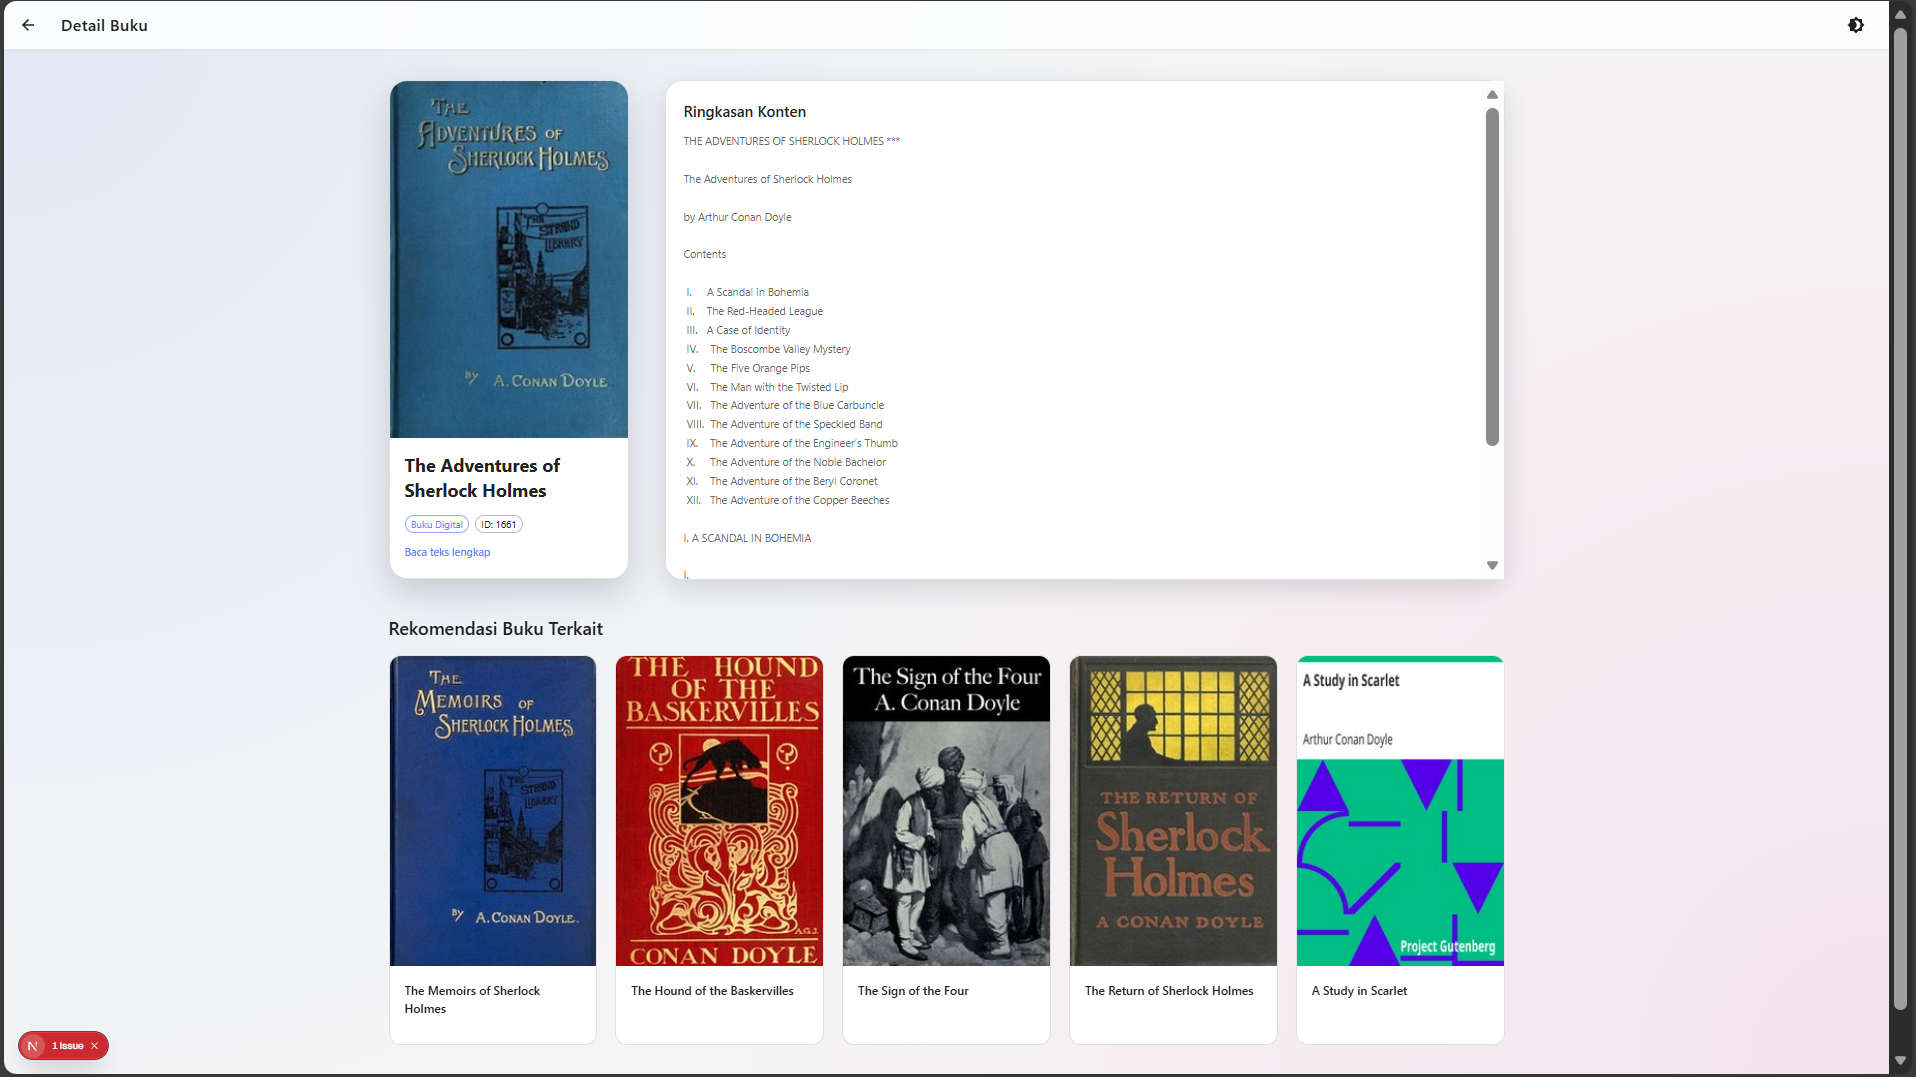
\includegraphics[width=0.75\textwidth]{img/eksperimen/rec/rec1.png}
    \caption{Hasil Rekomendasi Detail Buku \textit{The Adventure of Sherlock Holmes}.}
    \label{fig:rec-1}
\end{figure}

\begin{figure}[H]
    \centering
    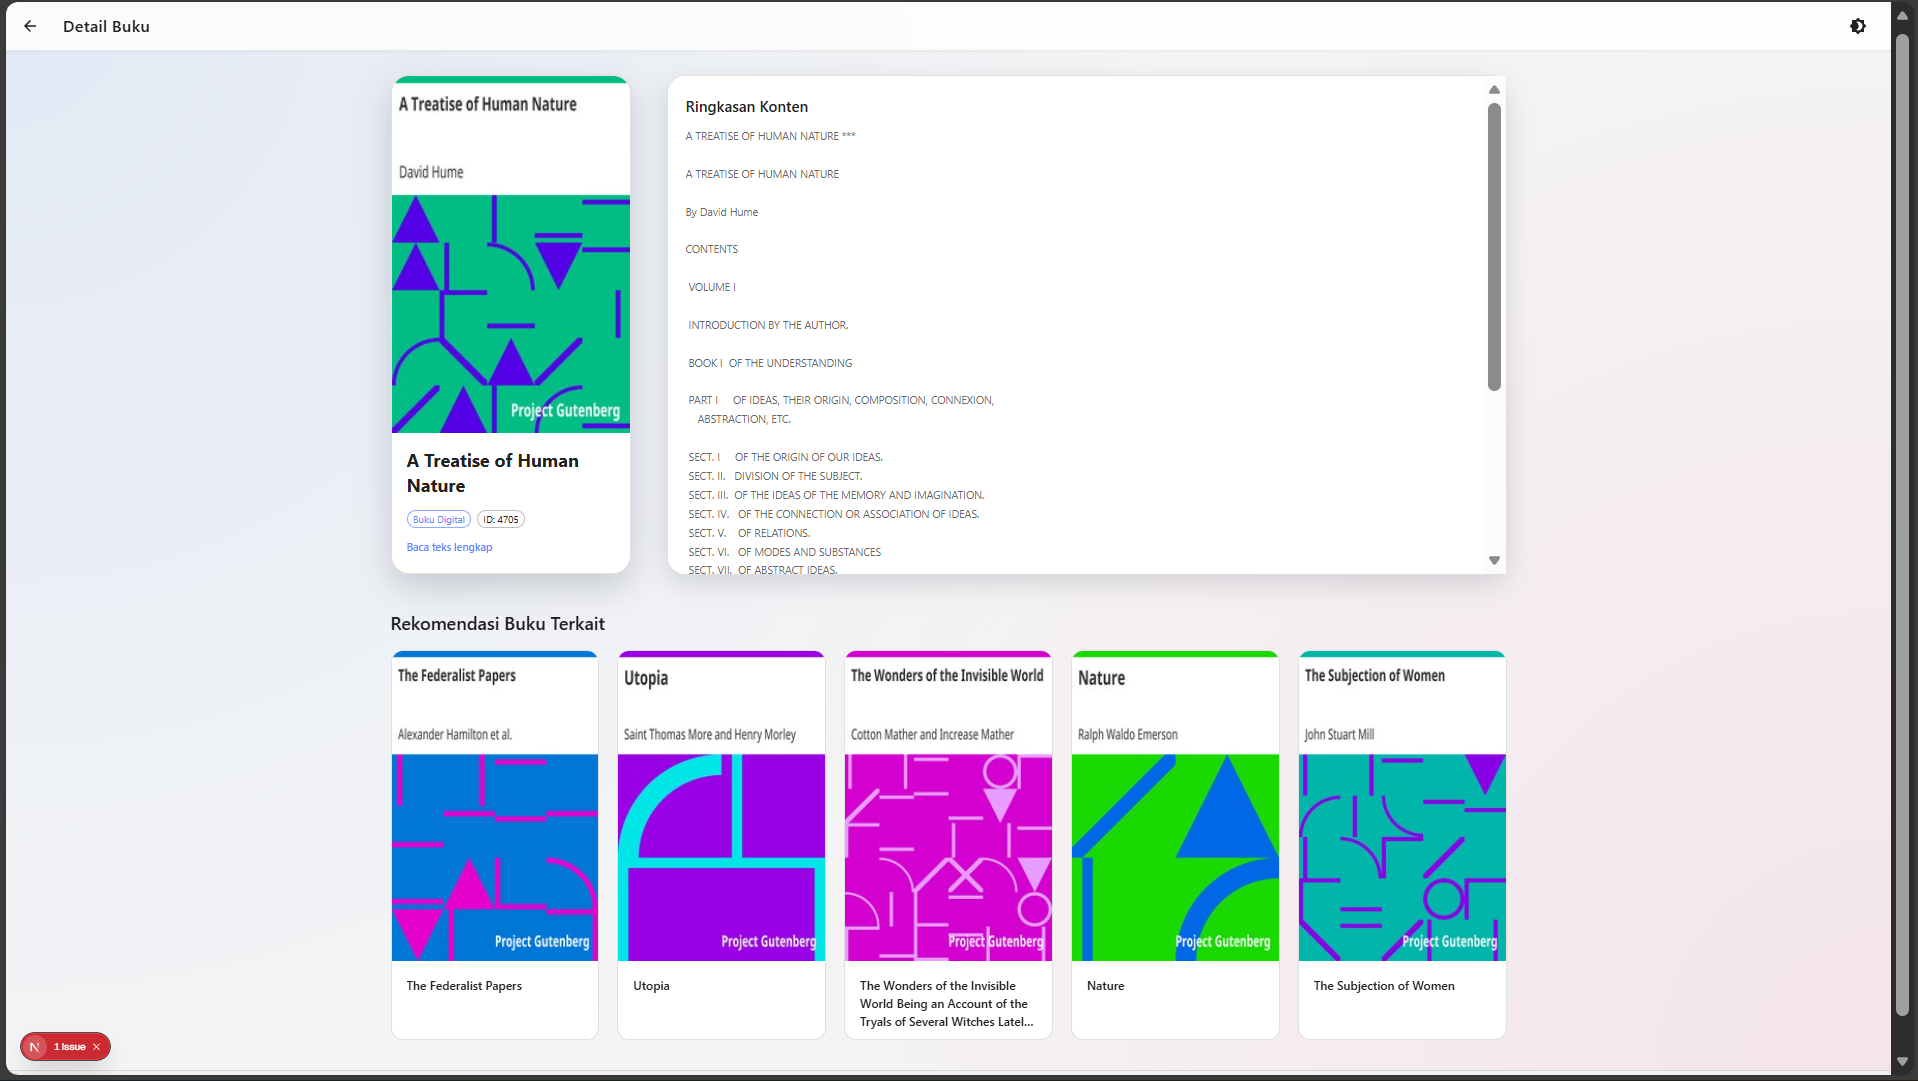
\includegraphics[width=0.75\textwidth]{img/eksperimen/rec/rec2.png}
    \caption{Hasil Rekomendasi Detail Buku \textit{A Treatise of Human Nature}.}
    \label{fig:rec-2}
\end{figure}

\textbf{Analisis Rekomendasi:}
\begin{enumerate}
\item \textbf{The Adventure of Sherlock Holmes} \\
    Pada pengujian pertama ini, penulis menemukan bahwa sistem bekerja sangat optimal. Hasil rekomendasi yang diberikan mencapai tingkat kecocokan sempurna, jika dibandingkan dengan referensi yang diberikan. Yang menarik, skor kemiripan (similarity score) antar-buku sangatlah tinggi, bahkan menembus angka 0.99. Hal ini menunjukkan bahwa algoritma LSA penulis berhasil "membaca" pola kata-kata yang unik, seperti kata "Holmes", "Watson", atau "Baker Street", dan menggunakannya untuk mengelompokkan buku-buku ini dalam satu kategori yang sangat rapat.

    \item \textbf{A Treatise of Human Nature} \\
    Hasil pada pengujian kedua ini cukup mengejutkan namun menarik untuk dianalisis. Meskipun judul buku yang direkomendasikan berbeda total dari referensi yang diberikan, rekomendasi yang diberikan sistem penulis sebenarnya masih sangat masuk akal secara konteks. Alih-alih mengarahkan ke buku filsafat ilmu (epistemologi) murni, sistem penulis sepertinya menangkap irisan topik yang lebih luas, yaitu tentang "Sifat Manusia" dalam konteks sosial dan politik. Hal ini terlihat dari munculnya buku seperti The Federalist Papers dan Utopia. Pergeseran ini bisa dimaklumi karena pemikiran Hume memang menjadi landasan bagi banyak teori politik modern. \\

    Selain itu, penulis juga menemukan satu buku outlier berjudul The Wonders of the Invisible World. Setelah penulis telusuri, masuknya buku ini kemungkinan besar disebabkan oleh kemiripan gaya bahasa (stylistic features). Kedua buku ini sama-sama menggunakan struktur kalimat dan kosa kata Inggris Klasik abad 17-18, sehingga sistem menganggap vektor kedua buku ini berdekatan, meskipun topik bahasannya sebenarnya berbeda.
\end{enumerate}

\subsubsection{Fitur \textit{Search by Document}}
Pengujian dilakukan dengan penulis melakukan uploading sebuah file.txt kedalam program dan kemudian memeriksa apakah hasil yang ditampilkan pada proram sesuai dengan konteks isi dari file.txt yang penulis kirim. Perlu diingat bahwa fitur \textit{search by document} ini berbasis LSA, bukan \textit{sub-string matching} seperti pada pencarian judul. Oleh karena itu konten yang ada di dalam file.txt akan di proses juga menggunakan LSA. Berikut adalah file.txt yang penulis gunakan untuk melakukan uji coba:

\begin{enumerate}
    \item {test1.txt}
    \begin{asciiBox}
    sherlock holmes mystery detective
    \end{asciiBox}
    \item {test2.txt}
    \begin{asciiBox}
    Alice was beginning to get very tired of sitting by her sister on the bank, and of having nothing to do: once or twice she had peeped into the book her sister was reading, but it had no pictures or conversations in it, “and what is the use of a book,” thought Alice “without pictures or conversations?”

    So she was considering in her own mind (as well as she could, for the hot day made her feel very sleepy and stupid), whether the pleasure of making a daisy-chain would be worth the trouble of getting up and picking the daisies, when suddenly a White Rabbit with pink eyes ran close by her.

    There was nothing so _very_ remarkable in that; nor did Alice think it so _very_ much out of the way to hear the Rabbit say to itself, “Oh dear! Oh dear! I shall be late!” (when she thought it over afterwards, it occurred to her that she ought to have wondered at this, but at the time it all seemed quite natural); but when the Rabbit actually _took a watch out of its waistcoat-pocket_, and looked at it, and then hurried on, Alice started to her feet, for it flashed across her mind that she had never before seen a rabbit with either a waistcoat-pocket, or a watch to take out of it, and burning with curiosity, she ran across the field after it, and fortunately was just in time to see it pop down a large rabbit-hole under the hedge....
    \end{asciiBox}
\end{enumerate}

Berikut adalah hasil yang didapatkan dari uji coba menggunakan file.txt diatas:

\begin{figure}[H]
    \centering
    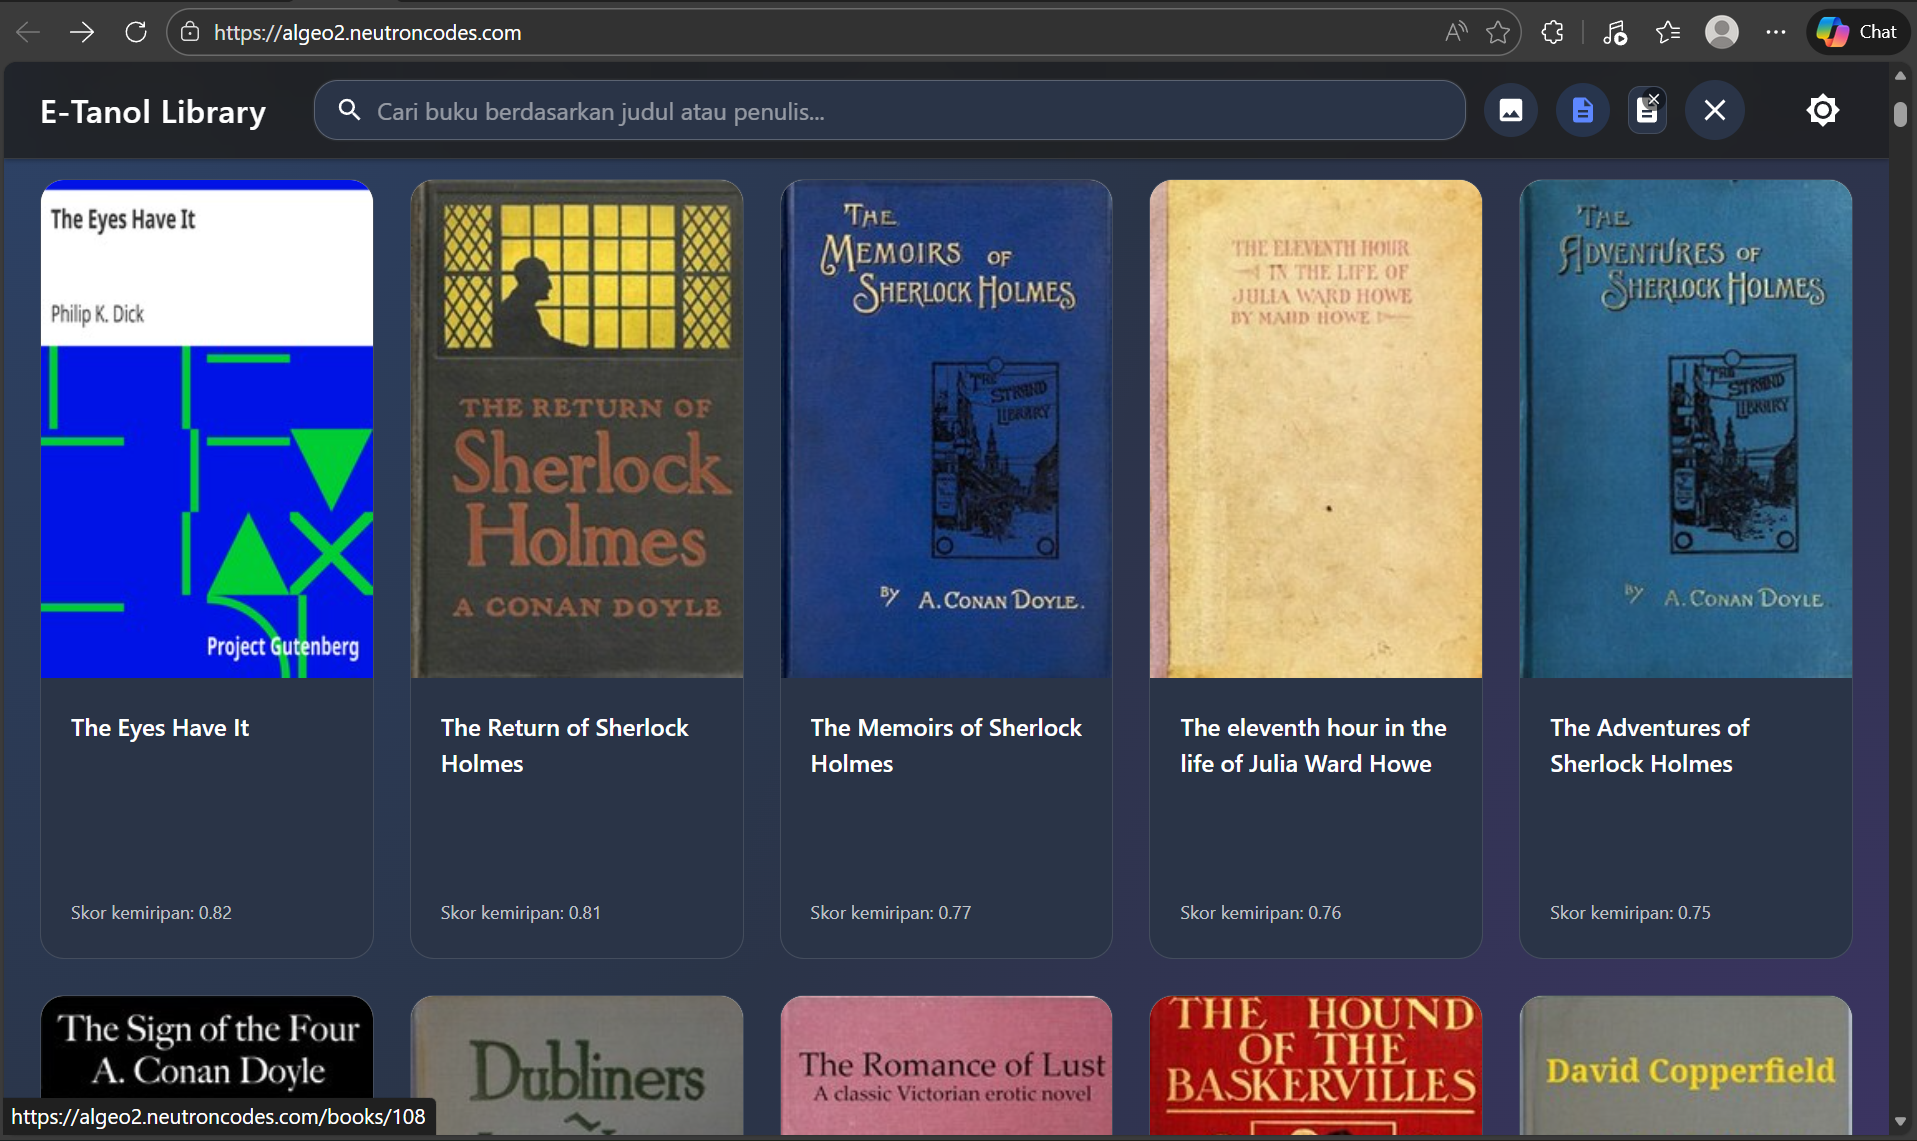
\includegraphics[width=0.75\textwidth]{img/eksperimen/rec/rec3.png}
    \caption{Hasil Search by Document \textit{test1.txt}.}
    \label{fig:rec-2}
\end{figure}

\begin{figure}[H]
    \centering
    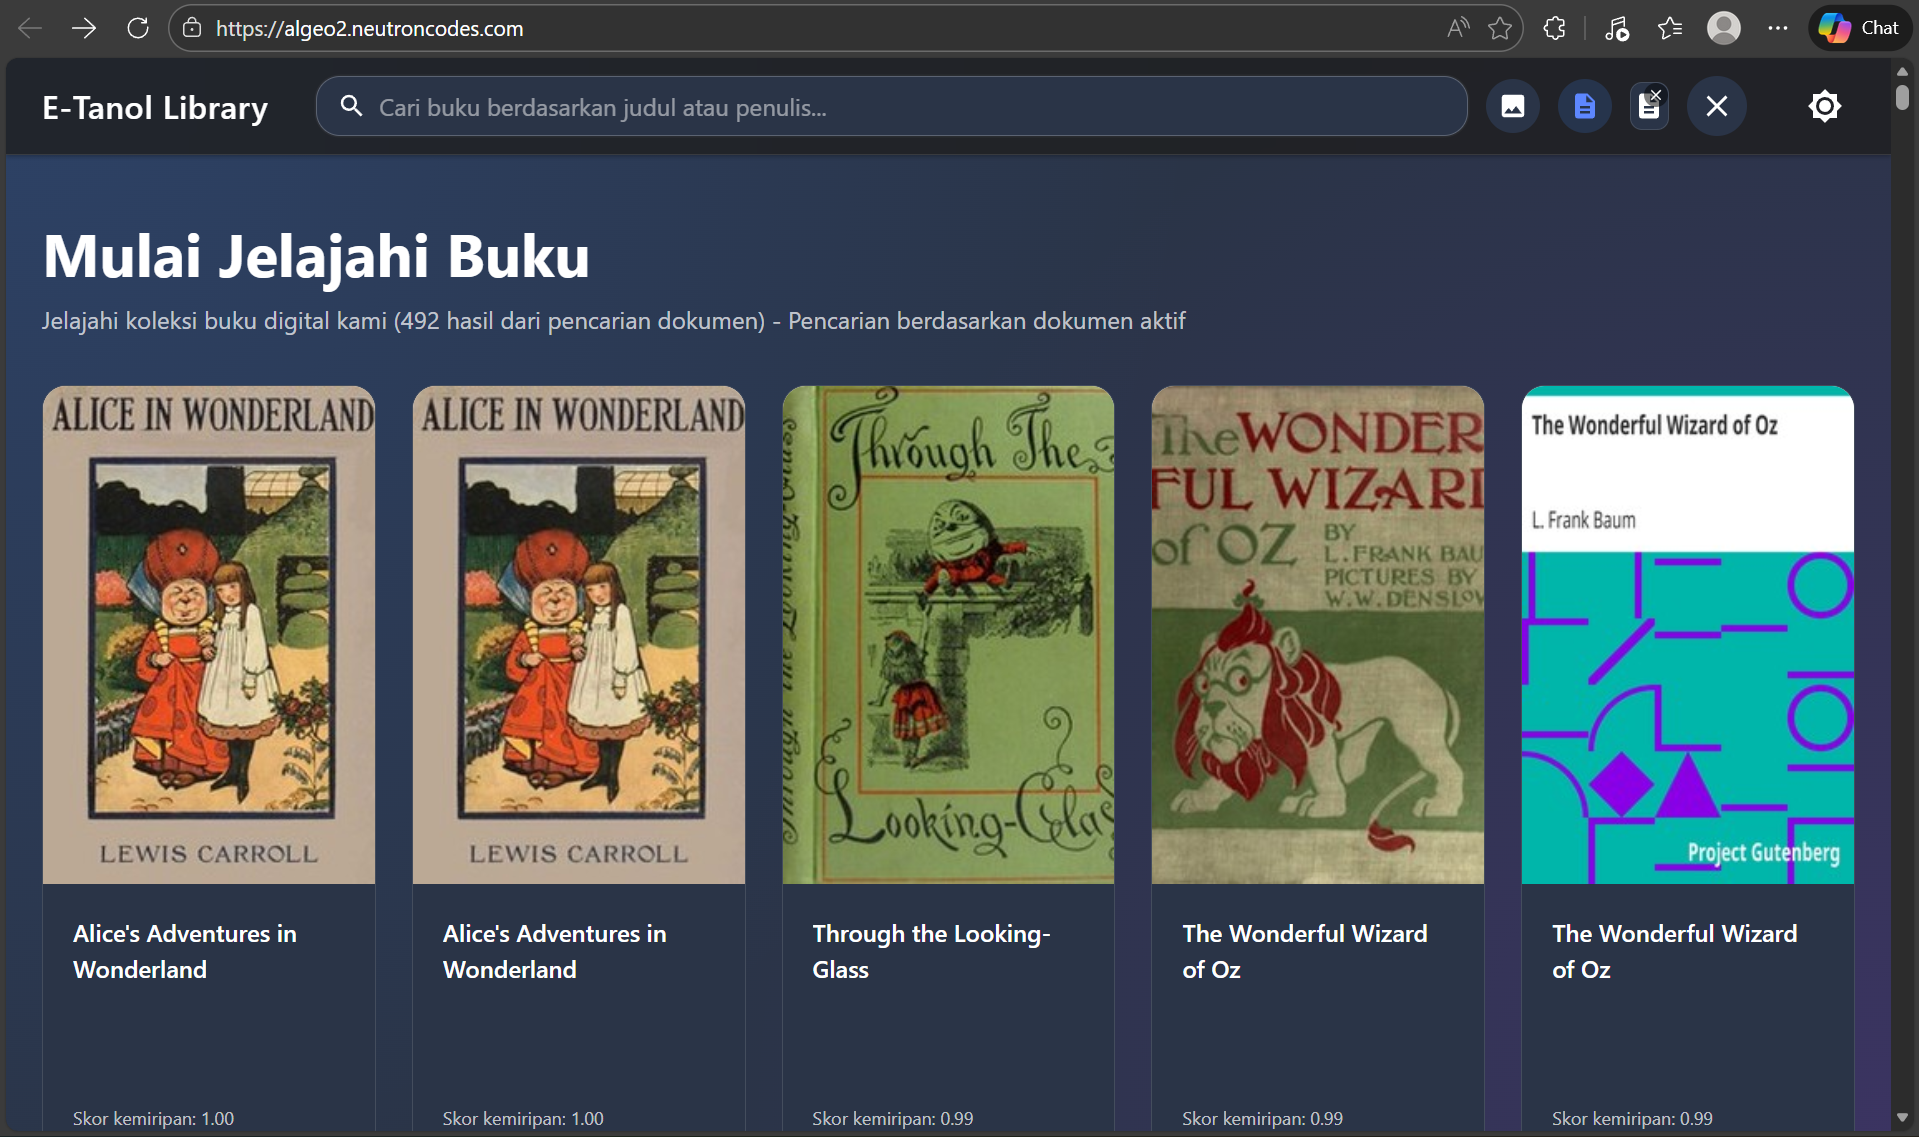
\includegraphics[width=0.75\textwidth]{img/eksperimen/rec/rec4.png}
    \caption{Hasil Search by Document \textit{test2.txt}.}
    \label{fig:rec-2}
\end{figure}

\textbf{Analisis Pencarian:}
\begin{enumerate}
\item \textbf{test1.txt} \\
    Pada pengujian pertama, kami menggunakan file.txt dengan isi konten yang pendek (hanya tiga kata). Kami menspesifikasikan isi konten dari file.txt agar terperinci di tiga hal, yaitu genre "mystery" dan "detective", dan hasil yang didapatkan cukup memuaskan, dimana buku incaran penulis (seri Sherlock Holmes) juga ada di dalam pencarian.

    \item \textbf{test2.txt} \\
    Pada pengujian kedua, kami menggunakan mekanisme yang sangat berbeda dibandingkan dengan pengujian pertama, yaitu kami mencoba melakukan search by document dengan isi file.txt adalah seluruh isi teks dari buku tertentu (Alice in Wonderland). Hasil yang didapatkan sangat memuaskan, buku yang memang isi dari file.txt penulis muncul sebagai urutan pertama dengan skor similaritas (1.0)
\end{enumerate}

% Bab 5 Penutup
\newpage
\section{Penutup}
\subsection{Kesimpulan}
Berdasarkan hasil implementasi dan pengujian sistem perpustakaan digital "E-TANOL" yang menerapkan konsep Aljabar Linier, dapat ditarik beberapa kesimpulan sebagai berikut:

\begin{enumerate}
    \item Keunggulan SVD pada Data Non-Persegi Penerapan \textit{Singular Value Decomposition} (SVD) terbukti lebih superior dan fleksibel dibandingkan \textit{Eigendecomposition} standar dalam konteks pengolahan data riil. Mengingat matriks data citra (sampul buku) dan dokumen yang dibangun memiliki dimensi $N \times M$ (persegi panjang), SVD mampu melakukan faktorisasi matriks secara langsung untuk mendapatkan basis ortonormal dan nilai singular tanpa batasan dimensi matriks, sehingga sangat cocok untuk ekstraksi fitur pada \textit{dataset} yang jumlah sampelnya tidak sama dengan jumlah fiturnya.
    \item Efektivitas \textit{Eigenfaces} dalam Temu Balik Citra Metode Eigenfaces (PCA via SVD) berhasil mengimplementasikan sistem pencarian citra yang efisien dengan memanfaatkan reduksi dimensi. Sistem mampu mengenali sampul buku berdasarkan pola visual globalnya dengan akurasi yang baik pada kondisi ideal. Namun, metode ini terbukti sensitif (kurang optimal) terhadap variasi geometris (seperti rotasi, pergeseran, atau \textit{cropping}) dan variasi pencahayaan ekstrem, karena algoritma bekerja berdasarkan perbandingan intensitas piksel pada koordinat yang kaku.
    \item Semantik Laten dalam Temu Balik Dokumen Pada pencarian teks, pemanfaatan nilai eigen dan vektor eigen berhasil menangkap hubungan semantik antar dokumen (\textit{Latent Semantic Indexing}). Hasil pengujian menunjukkan sistem mampu mengelompokkan dokumen berdasarkan genre dan nuansa cerita (seperti pengelompokan novel \textit{Sherlock Holmes} (latar \textit{Victorian}) dan literatur klasik filosofi dan filsafat (\textit{A Treatise of Human Nature})) bukan sekadar pencocokan kata kunci semata. Hal ini membuktikan bahwa vektor eigen mampu merepresentasikan fitur utama (topik) dari sekumpulan data teks.
    \item Efisiensi Komputasi dan Penyimpanan Penerapan teorema aproksimasi \textit{low-rank} (mengambil $k$ nilai singular terbesar) terbukti signifikan dalam menghemat ruang penyimpanan dan mempercepat waktu komputasi pencarian (\textit{query}). Dengan membuang komponen nilai singular yang kecil (dianggap sebagai \textit{noise}), sistem tetap dapat mempertahankan informasi esensial citra dan teks dengan ukuran data yang jauh lebih kecil dibandingkan data aslinya.
\end{enumerate}

\subsection{Saran Asisten}
\begin{itemize}
    \item \textbf{An-Dafa:}  Saya menyarankan adanya penekanan atau sumber daya tambahan mengenai metode numerik untuk pencarian eigenvalue dan eigenvector (seperti Power Iteration) karena pada implementasi menunjukkan bahwa dengan dataset dan matriks yang besar, menghitung eigenvalue atau eigenvector dengan cara yang diajarkan di kelas (QR Algorithm) sangatlah lama.
    \item \textbf{Haris:}  Testcase 3 \textit{Image Searching}, dataset \textit{image cover} yang sangat \textit{noise} dan terlalu terang tidak akan ditemukan tanpa preprocessing \textit{image} atau algoritma PCA yang lebih \textit{advance}.
    \item \textbf{Fazri:}  Penjelasan mengenai aturan bonus performa cepat kurang jelas karena setiap peserta mata kuliah mempunyai spek laptop yang berbeda-beda.
\end{itemize}

\subsection{Refleksi Pribadi Anggota Kelompok}
\begin{itemize}
    \item \textbf{An-Dafa:} Setelah saya mengerjakan Tugas Besar Aljabar Linear dan Geometri 2 ini saya memahami bahwa ilmu pengetahuan matematis, khususnya dalam komputer grafis sangatlah luas. Saya sangat 'salut' atas bagaimana manusia dapat menemukan semua perhitungan numerik yang kompleks ini hanya bermodalkan 'kayu' dan 'batu'. Selain itu saya juga terpukau dan bertanya-tanya "Wah bagaimana bisa mereka berpikir untuk menjadikan sebuah matriks sebagai dasar untuk melakukan image processing dan text processing?" tentunya hal tersebut sangatlah diluar nalar ketika kita throwback ke masa teknologi belum berkembang pesat seperti saat ini. 
    \item \textbf{Haris:} Pemahaman materi ternyata tidak cukup hanya dari teks dan gambar, visualisasi \textit{video} (seperti di youtube 3Blue1Brown\cite{3Blue1Brown}) ternyata sangat membantu agar saya bisa membayangkannya lebih jelas. 
    \item \textbf{Fazri:}  Saat mengerjakan bagian frontend, saya harus belajar kembali konsep responsif dalam web, kemudian saat mengintegrasikan algoritma pencarian saya harus belajar menyesuaikan waktu ketik realtime dengan call API agar tidak terjadi API flooding. 
\end{itemize}

% Daftar Pustaka
\newpage

\section*{Daftar Pustaka}
\addcontentsline{toc}{section}{Daftar Pustaka}

\bibliographystyle{IEEEtran}
\bibliography{daftar-pustaka}

% Lampiran
\newpage
\section*{Lampiran}
\addcontentsline{toc}{section}{Lampiran}

\begin{itemize}
    \item Tautan Repositori Github: \href{https://github.com/IRK-23/algeo2-e-tanol}{github.com/IRK-23/algeo2-e-tanol}
    \item Tautan Web: \href{https://algeo2.neutroncodes.com/}{algeo.neutroncode.com}
    \item Tautan Video Pengenalan Program: \href{https://youtu.be/4O_Qmi1UCMI}{ASEP BUKAN SEKEDAR PERFORMATIVE MALE?!}
\end{itemize}

\end{document}